\documentclass[1p]{elsarticle_modified}
%\bibliographystyle{elsarticle-num}

%\usepackage[colorlinks]{hyperref}
%\usepackage{abbrmath_seonhwa} %\Abb, \Ascr, \Acal ,\Abf, \Afrak
\usepackage{amsfonts}
\usepackage{amssymb}
\usepackage{amsmath}
\usepackage{amsthm}
\usepackage{scalefnt}
\usepackage{amsbsy}
\usepackage{kotex}
\usepackage{caption}
\usepackage{subfig}
\usepackage{color}
\usepackage{graphicx}
\usepackage{xcolor} %% white, black, red, green, blue, cyan, magenta, yellow
\usepackage{float}
\usepackage{setspace}
\usepackage{hyperref}

\usepackage{tikz}
\usetikzlibrary{arrows}

\usepackage{multirow}
\usepackage{array} % fixed length table
\usepackage{hhline}

%%%%%%%%%%%%%%%%%%%%%
\makeatletter
\renewcommand*\env@matrix[1][\arraystretch]{%
	\edef\arraystretch{#1}%
	\hskip -\arraycolsep
	\let\@ifnextchar\new@ifnextchar
	\array{*\c@MaxMatrixCols c}}
\makeatother %https://tex.stackexchange.com/questions/14071/how-can-i-increase-the-line-spacing-in-a-matrix
%%%%%%%%%%%%%%%

\usepackage[normalem]{ulem}

\newcommand{\msout}[1]{\ifmmode\text{\sout{\ensuremath{#1}}}\else\sout{#1}\fi}
%SOURCE: \msout is \stkout macro in https://tex.stackexchange.com/questions/20609/strikeout-in-math-mode

\newcommand{\cancel}[1]{
	\ifmmode
	{\color{red}\msout{#1}}
	\else
	{\color{red}\sout{#1}}
	\fi
}

\newcommand{\add}[1]{
	{\color{blue}\uwave{#1}}
}

\newcommand{\replace}[2]{
	\ifmmode
	{\color{red}\msout{#1}}{\color{blue}\uwave{#2}}
	\else
	{\color{red}\sout{#1}}{\color{blue}\uwave{#2}}
	\fi
}

\newcommand{\Sol}{\mathcal{S}} %segment
\newcommand{\D}{D} %diagram
\newcommand{\A}{\mathcal{A}} %arc


%%%%%%%%%%%%%%%%%%%%%%%%%%%%%5 test

\def\sl{\operatorname{\textup{SL}}(2,\Cbb)}
\def\psl{\operatorname{\textup{PSL}}(2,\Cbb)}
\def\quan{\mkern 1mu \triangleright \mkern 1mu}

\theoremstyle{definition}
\newtheorem{thm}{Theorem}[section]
\newtheorem{prop}[thm]{Proposition}
\newtheorem{lem}[thm]{Lemma}
\newtheorem{ques}[thm]{Question}
\newtheorem{cor}[thm]{Corollary}
\newtheorem{defn}[thm]{Definition}
\newtheorem{exam}[thm]{Example}
\newtheorem{rmk}[thm]{Remark}
\newtheorem{alg}[thm]{Algorithm}

\newcommand{\I}{\sqrt{-1}}
\begin{document}

%\begin{frontmatter}
%
%\title{Boundary parabolic representations of knots up to 8 crossings}
%
%%% Group authors per affiliation:
%\author{Yunhi Cho} 
%\address{Department of Mathematics, University of Seoul, Seoul, Korea}
%\ead{yhcho@uos.ac.kr}
%
%
%\author{Seonhwa Kim} %\fnref{s_kim}}
%\address{Center for Geometry and Physics, Institute for Basic Science, Pohang, 37673, Korea}
%\ead{ryeona17@ibs.re.kr}
%
%\author{Hyuk Kim}
%\address{Department of Mathematical Sciences, Seoul National University, Seoul 08826, Korea}
%\ead{hyukkim@snu.ac.kr}
%
%\author{Seokbeom Yoon}
%\address{Department of Mathematical Sciences, Seoul National University, Seoul, 08826,  Korea}
%\ead{sbyoon15@snu.ac.kr}
%
%\begin{abstract}
%We find all boundary parabolic representation of knots up to 8 crossings.
%
%\end{abstract}
%\begin{keyword}
%    \MSC[2010] 57M25 
%\end{keyword}
%
%\end{frontmatter}

%\linenumbers
%\tableofcontents
%
\newcommand\colored[1]{\textcolor{white}{\rule[-0.35ex]{0.8em}{1.4ex}}\kern-0.8em\color{red} #1}%
%\newcommand\colored[1]{\textcolor{white}{ #1}\kern-2.17ex	\textcolor{white}{ #1}\kern-1.81ex	\textcolor{white}{ #1}\kern-2.15ex\color{red}#1	}

{\Large $\underline{11a_{351}~(K11a_{351})}$}

\setlength{\tabcolsep}{10pt}
\renewcommand{\arraystretch}{1.6}
\vspace{1cm}\begin{tabular}{m{100pt}>{\centering\arraybackslash}m{274pt}}
\multirow{5}{120pt}{
	\centering
	\includegraphics[width=112pt]{../../../GIT/diagram.site/Diagrams/png/600_11a_351.png}\\
\ \ \ A knot diagram\footnotemark}&
\allowdisplaybreaks
\textbf{Linearized knot diagam} \\
\cline{2-2}
 &
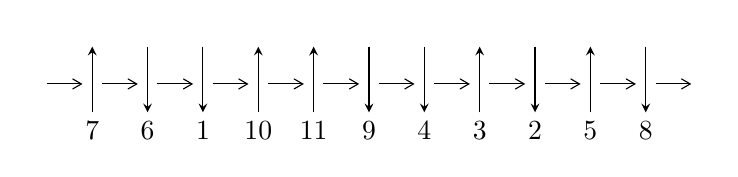
\begin{tikzpicture}[x=20pt, y=17pt]
	% nodes
	\node (C0) at (0, 0) {};
	\node (C1) at (1, 0) {};
	\node (C1U) at (1, +1) {};
	\node (C1D) at (1, -1) {7};

	\node (C2) at (2, 0) {};
	\node (C2U) at (2, +1) {};
	\node (C2D) at (2, -1) {6};

	\node (C3) at (3, 0) {};
	\node (C3U) at (3, +1) {};
	\node (C3D) at (3, -1) {1};

	\node (C4) at (4, 0) {};
	\node (C4U) at (4, +1) {};
	\node (C4D) at (4, -1) {10};

	\node (C5) at (5, 0) {};
	\node (C5U) at (5, +1) {};
	\node (C5D) at (5, -1) {11};

	\node (C6) at (6, 0) {};
	\node (C6U) at (6, +1) {};
	\node (C6D) at (6, -1) {9};

	\node (C7) at (7, 0) {};
	\node (C7U) at (7, +1) {};
	\node (C7D) at (7, -1) {4};

	\node (C8) at (8, 0) {};
	\node (C8U) at (8, +1) {};
	\node (C8D) at (8, -1) {3};

	\node (C9) at (9, 0) {};
	\node (C9U) at (9, +1) {};
	\node (C9D) at (9, -1) {2};

	\node (C10) at (10, 0) {};
	\node (C10U) at (10, +1) {};
	\node (C10D) at (10, -1) {5};

	\node (C11) at (11, 0) {};
	\node (C11U) at (11, +1) {};
	\node (C11D) at (11, -1) {8};
	\node (C12) at (12, 0) {};

	% arrows
	\draw[->,>={angle 60}]
	(C0) edge (C1) (C1) edge (C2) (C2) edge (C3) (C3) edge (C4) (C4) edge (C5) (C5) edge (C6) (C6) edge (C7) (C7) edge (C8) (C8) edge (C9) (C9) edge (C10) (C10) edge (C11) (C11) edge (C12) ;	\draw[->,>=stealth]
	(C1D) edge (C1U) (C2U) edge (C2D) (C3U) edge (C3D) (C4D) edge (C4U) (C5D) edge (C5U) (C6U) edge (C6D) (C7U) edge (C7D) (C8D) edge (C8U) (C9U) edge (C9D) (C10D) edge (C10U) (C11U) edge (C11D) ;
	\end{tikzpicture} \\
\hhline{~~} \\& 
\textbf{Solving Sequence} \\ \cline{2-2} 
 &
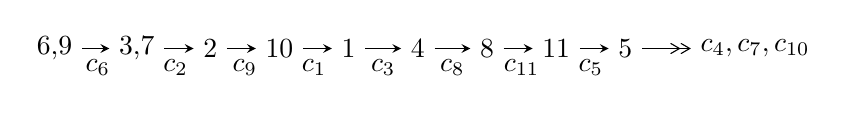
\begin{tikzpicture}[x=25pt, y=7pt]
	% node
	\node (A0) at (-1/8, 0) {6,9};
	\node (A1) at (17/16, 0) {3,7};
	\node (A2) at (17/8, 0) {2};
	\node (A3) at (25/8, 0) {10};
	\node (A4) at (33/8, 0) {1};
	\node (A5) at (41/8, 0) {4};
	\node (A6) at (49/8, 0) {8};
	\node (A7) at (57/8, 0) {11};
	\node (A8) at (65/8, 0) {5};
	\node (C1) at (1/2, -1) {$c_{6}$};
	\node (C2) at (13/8, -1) {$c_{2}$};
	\node (C3) at (21/8, -1) {$c_{9}$};
	\node (C4) at (29/8, -1) {$c_{1}$};
	\node (C5) at (37/8, -1) {$c_{3}$};
	\node (C6) at (45/8, -1) {$c_{8}$};
	\node (C7) at (53/8, -1) {$c_{11}$};
	\node (C8) at (61/8, -1) {$c_{5}$};
	\node (A9) at (10, 0) {$c_{4},c_{7},c_{10}$};

	% edge
	\draw[->,>=stealth]	
	(A0) edge (A1) (A1) edge (A2) (A2) edge (A3) (A3) edge (A4) (A4) edge (A5) (A5) edge (A6) (A6) edge (A7) (A7) edge (A8) ;
	\draw[->>,>={angle 60}]	
	(A8) edge (A9);
\end{tikzpicture} \\ 

\end{tabular} \\

\footnotetext{
The image of knot diagram is generated by the software ``\textbf{Draw programme}" developed by Andrew Bartholomew(\url{http://www.layer8.co.uk/maths/draw/index.htm\#Running-draw}), where we modified some parts for our purpose(\url{https://github.com/CATsTAILs/LinksPainter}).
}\phantom \\ \newline 
\centering \textbf{Ideals for irreducible components\footnotemark of $X_{\text{par}}$} 
 
\begin{align*}
I^u_{1}&=\langle 
5 u^{15}+60 u^{14}+\cdots+b+130,\;35 u^{15}+195 u^{14}+\cdots+19 a-844,\;u^{16}+11 u^{15}+\cdots+85 u+19\rangle \\
I^u_{2}&=\langle 
4 u^{11}+38 u^{10}+\cdots+b+71,\;3 u^{11}-4 u^{10}+\cdots+17 a-272,\;u^{12}+10 u^{11}+\cdots+102 u+17\rangle \\
I^u_{3}&=\langle 
-779024089 a^9 u-1957109432 a^8 u+\cdots+3952254721 a+13062915505,\\
\phantom{I^u_{3}}&\phantom{= \langle  }2 a^9 u+3 a^8 u+\cdots-24 a^2-5,\;u^2- u+1\rangle \\
I^u_{4}&=\langle 
10206521 a^9 u^3+21936282 a^8 u^3+\cdots-55249693 a-29498003,\;a^9 u^3-7 a^8 u^3+\cdots+50 a+317,\\
\phantom{I^u_{4}}&\phantom{= \langle  }u^4- u^3+2 u+1\rangle \\
I^u_{5}&=\langle 
9901203 u^{19}-97655512 u^{18}+\cdots+45127189 b-2967898,\\
\phantom{I^u_{5}}&\phantom{= \langle  }-6933305 u^{19}+80845633 u^{18}+\cdots+45127189 a-67619382,\;u^{20}-9 u^{19}+\cdots-3 u^2+1\rangle \\
I^u_{6}&=\langle 
- a^4- a^2+b+a,\;a^5+a^4+2 a^3+a^2+a+1,\;u-1\rangle \\
I^u_{7}&=\langle 
a^4+a^2+b,\;a^5+a^4+2 a^3+a^2+a+1,\;u-1\rangle \\
I^u_{8}&=\langle 
b+1,\;a,\;u-1\rangle \\
\\
I^v_{1}&=\langle 
a,\;b^5- b^4+2 b^3- b^2+b-1,\;v-1\rangle \\
\end{align*}
\raggedright * 9 irreducible components of $\dim_{\mathbb{C}}=0$, with total 124 representations.\\
\footnotetext{All coefficients of polynomials are rational numbers. But the coefficients are sometimes approximated in decimal forms when there is not enough margin.}
\newpage
\renewcommand{\arraystretch}{1}
\centering \section*{I. $I^u_{1}= \langle 5 u^{15}+60 u^{14}+\cdots+b+130,\;35 u^{15}+195 u^{14}+\cdots+19 a-844,\;u^{16}+11 u^{15}+\cdots+85 u+19 \rangle$}
\flushleft \textbf{(i) Arc colorings}\\
\begin{tabular}{m{7pt} m{180pt} m{7pt} m{180pt} }
\flushright $a_{6}=$&$\begin{pmatrix}1\\0\end{pmatrix}$ \\
\flushright $a_{9}=$&$\begin{pmatrix}0\\u\end{pmatrix}$ \\
\flushright $a_{3}=$&$\begin{pmatrix}-1.84211 u^{15}-10.2632 u^{14}+\cdots+138.789 u+44.4211\\-5 u^{15}-60 u^{14}+\cdots-496 u-130\end{pmatrix}$ \\
\flushright $a_{7}=$&$\begin{pmatrix}1\\u^2\end{pmatrix}$ \\
\flushright $a_{2}=$&$\begin{pmatrix}-6.84211 u^{15}-70.2632 u^{14}+\cdots-357.211 u-85.5789\\-5 u^{15}-60 u^{14}+\cdots-496 u-130\end{pmatrix}$ \\
\flushright $a_{10}=$&$\begin{pmatrix}0.473684 u^{15}+4.21053 u^{14}+\cdots-2.63158 u-2.73684\\u^{15}+10 u^{14}+\cdots+44 u+9\end{pmatrix}$ \\
\flushright $a_{1}=$&$\begin{pmatrix}3.15789 u^{15}+20.7368 u^{14}+\cdots-156.211 u-50.5789\\15 u^{15}+160 u^{14}+\cdots+929 u+231\end{pmatrix}$ \\
\flushright $a_{4}=$&$\begin{pmatrix}12.1579 u^{15}+118.737 u^{14}+\cdots+457.789 u+104.421\\21 u^{14}+180 u^{13}+\cdots+548 u+155\end{pmatrix}$ \\
\flushright $a_{8}=$&$\begin{pmatrix}-0.526316 u^{15}-4.78947 u^{14}+\cdots-12.6316 u-1.73684\\- u^{14}-9 u^{13}+\cdots-32 u-10\end{pmatrix}$ \\
\flushright $a_{11}=$&$\begin{pmatrix}2.57895 u^{15}+37.3684 u^{14}+\cdots+428.895 u+117.211\\-10 u^{15}-94 u^{14}+\cdots-302 u-65\end{pmatrix}$ \\
\flushright $a_{5}=$&$\begin{pmatrix}-1.63158 u^{15}-23.9474 u^{14}+\cdots-287.158 u-77.6842\\7 u^{15}+71 u^{14}+\cdots+343 u+83\end{pmatrix}$\\ \flushright $a_{5}=$&$\begin{pmatrix}-1.63158 u^{15}-23.9474 u^{14}+\cdots-287.158 u-77.6842\\7 u^{15}+71 u^{14}+\cdots+343 u+83\end{pmatrix}$\\&\end{tabular}
\flushleft \textbf{(ii) Obstruction class $= -1$}\\~\\
\flushleft \textbf{(iii) Cusp Shapes $= 20 u^{15}+204 u^{14}+914 u^{13}+2234 u^{12}+2754 u^{11}-94 u^{10}-6024 u^9-9048 u^8-3284 u^7+8196 u^6+15768 u^5+14640 u^4+8642 u^3+3488 u^2+1062 u+264$}\\~\\
\newpage\renewcommand{\arraystretch}{1}
\flushleft \textbf{(iv) u-Polynomials at the component}\newline \\
\begin{tabular}{m{50pt}|m{274pt}}
Crossings & \hspace{64pt}u-Polynomials at each crossing \\
\hline $$\begin{aligned}c_{1},c_{8}\end{aligned}$$&$\begin{aligned}
&u^{16}+u^{15}+\cdots+2 u+2
\end{aligned}$\\
\hline $$\begin{aligned}c_{2},c_{7},c_{9}\\c_{11}\end{aligned}$$&$\begin{aligned}
&u^{16}+u^{15}+\cdots+u+1
\end{aligned}$\\
\hline $$\begin{aligned}c_{3},c_{6}\end{aligned}$$&$\begin{aligned}
&u^{16}-11 u^{15}+\cdots-85 u+19
\end{aligned}$\\
\hline $$\begin{aligned}c_{4},c_{5},c_{10}\end{aligned}$$&$\begin{aligned}
&u^{16}+6 u^{15}+\cdots+8 u+8
\end{aligned}$\\
\hline
\end{tabular}\\~\\
\newpage\renewcommand{\arraystretch}{1}
\flushleft \textbf{(v) Riley Polynomials at the component}\newline \\
\begin{tabular}{m{50pt}|m{274pt}}
Crossings & \hspace{64pt}Riley Polynomials at each crossing \\
\hline $$\begin{aligned}c_{1},c_{8}\end{aligned}$$&$\begin{aligned}
&y^{16}+9 y^{15}+\cdots+48 y+4
\end{aligned}$\\
\hline $$\begin{aligned}c_{2},c_{7},c_{9}\\c_{11}\end{aligned}$$&$\begin{aligned}
&y^{16}+7 y^{15}+\cdots+21 y+1
\end{aligned}$\\
\hline $$\begin{aligned}c_{3},c_{6}\end{aligned}$$&$\begin{aligned}
&y^{16}-11 y^{15}+\cdots+3795 y+361
\end{aligned}$\\
\hline $$\begin{aligned}c_{4},c_{5},c_{10}\end{aligned}$$&$\begin{aligned}
&y^{16}-12 y^{15}+\cdots+160 y+64
\end{aligned}$\\
\hline
\end{tabular}\\~\\
\newpage\flushleft \textbf{(vi) Complex Volumes and Cusp Shapes}
$$\begin{array}{c|c|c}  
\text{Solutions to }I^u_{1}& \I (\text{vol} + \sqrt{-1}CS) & \text{Cusp shape}\\
 \hline 
\begin{aligned}
u &= -0.380977 + 0.787211 I \\
a &= -1.029130 - 0.000584 I \\
b &= \phantom{-}0.393453 + 0.808033 I\end{aligned}
 & \phantom{-}5.25768 - 4.77897 I & \phantom{-}4.31247 + 4.75614 I \\ \hline\begin{aligned}
u &= -0.380977 - 0.787211 I \\
a &= -1.029130 + 0.000584 I \\
b &= \phantom{-}0.393453 - 0.808033 I\end{aligned}
 & \phantom{-}5.25768 + 4.77897 I & \phantom{-}4.31247 - 4.75614 I \\ \hline\begin{aligned}
u &= \phantom{-}1.279880 + 0.358721 I \\
a &= \phantom{-}0.170555 + 0.671225 I \\
b &= -0.052349 - 0.395411 I\end{aligned}
 & -2.56459 - 2.34570 I & -6.28872 + 0.46963 I \\ \hline\begin{aligned}
u &= \phantom{-}1.279880 - 0.358721 I \\
a &= \phantom{-}0.170555 - 0.671225 I \\
b &= -0.052349 + 0.395411 I\end{aligned}
 & -2.56459 + 2.34570 I & -6.28872 - 0.46963 I \\ \hline\begin{aligned}
u &= -1.22875 + 0.75885 I \\
a &= \phantom{-}0.284860 + 0.655547 I \\
b &= \phantom{-}0.403315 - 1.238380 I\end{aligned}
 & \phantom{-}8.29097 + 6.33547 I & \phantom{-}5.46130 - 6.31546 I \\ \hline\begin{aligned}
u &= -1.22875 - 0.75885 I \\
a &= \phantom{-}0.284860 - 0.655547 I \\
b &= \phantom{-}0.403315 + 1.238380 I\end{aligned}
 & \phantom{-}8.29097 - 6.33547 I & \phantom{-}5.46130 + 6.31546 I \\ \hline\begin{aligned}
u &= -1.16827 + 1.01352 I \\
a &= \phantom{-}0.104611 - 1.132590 I \\
b &= -1.20879 + 1.21269 I\end{aligned}
 & \phantom{-}2.8802 + 18.5253 I & \phantom{-}0.82769 - 9.63606 I \\ \hline\begin{aligned}
u &= -1.16827 - 1.01352 I \\
a &= \phantom{-}0.104611 + 1.132590 I \\
b &= -1.20879 - 1.21269 I\end{aligned}
 & \phantom{-}2.8802 - 18.5253 I & \phantom{-}0.82769 + 9.63606 I \\ \hline\begin{aligned}
u &= -1.54277 + 0.30640 I \\
a &= -0.064517 - 0.349095 I \\
b &= -0.120682 + 0.887722 I\end{aligned}
 & -0.76511 + 3.23091 I & \phantom{-}8.87467 - 5.88690 I \\ \hline\begin{aligned}
u &= -1.54277 - 0.30640 I \\
a &= -0.064517 + 0.349095 I \\
b &= -0.120682 - 0.887722 I\end{aligned}
 & -0.76511 - 3.23091 I & \phantom{-}8.87467 + 5.88690 I\\
 \hline 
 \end{array}$$\newpage$$\begin{array}{c|c|c}  
\text{Solutions to }I^u_{1}& \I (\text{vol} + \sqrt{-1}CS) & \text{Cusp shape}\\
 \hline 
\begin{aligned}
u &= -1.20852 + 1.02268 I \\
a &= -0.121691 + 1.002120 I \\
b &= \phantom{-}1.08577 - 1.07970 I\end{aligned}
 & -2.9800 + 13.9622 I & -2.59981 - 9.26713 I \\ \hline\begin{aligned}
u &= -1.20852 - 1.02268 I \\
a &= -0.121691 - 1.002120 I \\
b &= \phantom{-}1.08577 + 1.07970 I\end{aligned}
 & -2.9800 - 13.9622 I & -2.59981 + 9.26713 I \\ \hline\begin{aligned}
u &= \phantom{-}0.035423 + 0.412947 I \\
a &= \phantom{-}1.80300 + 0.46760 I \\
b &= -0.145251 - 0.677138 I\end{aligned}
 & \phantom{-}0.27480 - 1.44128 I & \phantom{-}1.93375 + 5.30960 I \\ \hline\begin{aligned}
u &= \phantom{-}0.035423 - 0.412947 I \\
a &= \phantom{-}1.80300 - 0.46760 I \\
b &= -0.145251 + 0.677138 I\end{aligned}
 & \phantom{-}0.27480 + 1.44128 I & \phantom{-}1.93375 - 5.30960 I \\ \hline\begin{aligned}
u &= -1.28602 + 0.99596 I \\
a &= \phantom{-}0.062844 - 0.836469 I \\
b &= -0.855461 + 1.000990 I\end{aligned}
 & -1.34679 + 8.40080 I & -0.52134 - 6.47139 I \\ \hline\begin{aligned}
u &= -1.28602 - 0.99596 I \\
a &= \phantom{-}0.062844 + 0.836469 I \\
b &= -0.855461 - 1.000990 I\end{aligned}
 & -1.34679 - 8.40080 I & -0.52134 + 6.47139 I\\
 \hline 
 \end{array}$$\newpage\newpage\renewcommand{\arraystretch}{1}
\centering \section*{II. $I^u_{2}= \langle 4 u^{11}+38 u^{10}+\cdots+b+71,\;3 u^{11}-4 u^{10}+\cdots+17 a-272,\;u^{12}+10 u^{11}+\cdots+102 u+17 \rangle$}
\flushleft \textbf{(i) Arc colorings}\\
\begin{tabular}{m{7pt} m{180pt} m{7pt} m{180pt} }
\flushright $a_{6}=$&$\begin{pmatrix}1\\0\end{pmatrix}$ \\
\flushright $a_{9}=$&$\begin{pmatrix}0\\u\end{pmatrix}$ \\
\flushright $a_{3}=$&$\begin{pmatrix}-0.176471 u^{11}+0.235294 u^{10}+\cdots+70.2353 u+16\\-4 u^{11}-38 u^{10}+\cdots-371 u-71\end{pmatrix}$ \\
\flushright $a_{7}=$&$\begin{pmatrix}1\\u^2\end{pmatrix}$ \\
\flushright $a_{2}=$&$\begin{pmatrix}-4.17647 u^{11}-37.7647 u^{10}+\cdots-300.765 u-55\\-4 u^{11}-38 u^{10}+\cdots-371 u-71\end{pmatrix}$ \\
\flushright $a_{10}=$&$\begin{pmatrix}-1.47059 u^{11}-12.7059 u^{10}+\cdots-80.7059 u-13\\-2 u^{11}-18 u^{10}+\cdots-136 u-25\end{pmatrix}$ \\
\flushright $a_{1}=$&$\begin{pmatrix}-2.17647 u^{11}-21.7647 u^{10}+\cdots-266.765 u-52\\u^{11}+8 u^{10}+\cdots+3 u-3\end{pmatrix}$ \\
\flushright $a_{4}=$&$\begin{pmatrix}-8.17647 u^{11}-71.7647 u^{10}+\cdots-476.765 u-83\\-7 u^{11}-67 u^{10}+\cdots-714 u-139\end{pmatrix}$ \\
\flushright $a_{8}=$&$\begin{pmatrix}0.529412 u^{11}+4.29412 u^{10}+\cdots+14.2941 u+3\\u^{10}+8 u^9+\cdots+43 u+9\end{pmatrix}$ \\
\flushright $a_{11}=$&$\begin{pmatrix}-1.76471 u^{11}-19.6471 u^{10}+\cdots-338.647 u-68\\3 u^{11}+26 u^{10}+\cdots+136 u+21\end{pmatrix}$ \\
\flushright $a_{5}=$&$\begin{pmatrix}-0.0588235 u^{11}+2.41176 u^{10}+\cdots+156.412 u+35\\-4 u^{11}-36 u^{10}+\cdots-289 u-52\end{pmatrix}$\\ \flushright $a_{5}=$&$\begin{pmatrix}-0.0588235 u^{11}+2.41176 u^{10}+\cdots+156.412 u+35\\-4 u^{11}-36 u^{10}+\cdots-289 u-52\end{pmatrix}$\\&\end{tabular}
\flushleft \textbf{(ii) Obstruction class $= -1$}\\~\\
\flushleft \textbf{(iii) Cusp Shapes $= -15 u^{11}-131 u^{10}-625 u^9-1949 u^8-4347 u^7-7138 u^6-8765 u^5-8007 u^4-5383 u^3-2560 u^2-816 u-127$}\\~\\
\newpage\renewcommand{\arraystretch}{1}
\flushleft \textbf{(iv) u-Polynomials at the component}\newline \\
\begin{tabular}{m{50pt}|m{274pt}}
Crossings & \hspace{64pt}u-Polynomials at each crossing \\
\hline $$\begin{aligned}c_{1},c_{8}\end{aligned}$$&$\begin{aligned}
&(u^6- u^4+u^3+u^2-1)^2
\end{aligned}$\\
\hline $$\begin{aligned}c_{2},c_{7},c_{9}\\c_{11}\end{aligned}$$&$\begin{aligned}
&u^{12}+u^{10}- u^9+8 u^8+u^7+8 u^6-8 u^5+4 u^4+u^3+4 u^2-3 u+1
\end{aligned}$\\
\hline $$\begin{aligned}c_{3},c_{6}\end{aligned}$$&$\begin{aligned}
&u^{12}-10 u^{11}+\cdots-102 u+17
\end{aligned}$\\
\hline $$\begin{aligned}c_{4},c_{5},c_{10}\end{aligned}$$&$\begin{aligned}
&(u^6+3 u^5+2 u^4+u^2-2 u-4)^2
\end{aligned}$\\
\hline
\end{tabular}\\~\\
\newpage\renewcommand{\arraystretch}{1}
\flushleft \textbf{(v) Riley Polynomials at the component}\newline \\
\begin{tabular}{m{50pt}|m{274pt}}
Crossings & \hspace{64pt}Riley Polynomials at each crossing \\
\hline $$\begin{aligned}c_{1},c_{8}\end{aligned}$$&$\begin{aligned}
&(y^6-2 y^5+3 y^4-5 y^3+3 y^2-2 y+1)^2
\end{aligned}$\\
\hline $$\begin{aligned}c_{2},c_{7},c_{9}\\c_{11}\end{aligned}$$&$\begin{aligned}
&y^{12}+2 y^{11}+\cdots- y+1
\end{aligned}$\\
\hline $$\begin{aligned}c_{3},c_{6}\end{aligned}$$&$\begin{aligned}
&y^{12}+6 y^{11}+\cdots+918 y+289
\end{aligned}$\\
\hline $$\begin{aligned}c_{4},c_{5},c_{10}\end{aligned}$$&$\begin{aligned}
&(y^6-5 y^5+6 y^4+8 y^3-15 y^2-12 y+16)^2
\end{aligned}$\\
\hline
\end{tabular}\\~\\
\newpage\flushleft \textbf{(vi) Complex Volumes and Cusp Shapes}
$$\begin{array}{c|c|c}  
\text{Solutions to }I^u_{2}& \I (\text{vol} + \sqrt{-1}CS) & \text{Cusp shape}\\
 \hline 
\begin{aligned}
u &= -1.014560 + 0.523445 I \\
a &= -0.208887 - 0.713790 I \\
b &= -1.14261 + 1.15043 I\end{aligned}
 & -1.71358 + 4.97819 I & \phantom{-}0.7768 - 21.8821 I \\ \hline\begin{aligned}
u &= -1.014560 - 0.523445 I \\
a &= -0.208887 + 0.713790 I \\
b &= -1.14261 - 1.15043 I\end{aligned}
 & -1.71358 - 4.97819 I & \phantom{-}0.7768 + 21.8821 I \\ \hline\begin{aligned}
u &= -0.681059 + 0.947774 I \\
a &= -0.626037 - 0.871204 I \\
b &= -0.399338 + 1.186680 I\end{aligned}
 & \phantom{-}10.0009\phantom{ +0.000000I} & \phantom{-}7.28456 + 0. I\phantom{ +0.000000I} \\ \hline\begin{aligned}
u &= -0.681059 - 0.947774 I \\
a &= -0.626037 + 0.871204 I \\
b &= -0.399338 - 1.186680 I\end{aligned}
 & \phantom{-}10.0009\phantom{ +0.000000I} & \phantom{-}7.28456 + 0. I\phantom{ +0.000000I} \\ \hline\begin{aligned}
u &= -1.011620 + 0.702683 I \\
a &= \phantom{-}0.146588 + 0.944898 I \\
b &= \phantom{-}1.19430 - 1.17568 I\end{aligned}
 & \phantom{-}3.78738 + 10.11610 I & \phantom{-}0.74000 - 10.55076 I \\ \hline\begin{aligned}
u &= -1.011620 - 0.702683 I \\
a &= \phantom{-}0.146588 - 0.944898 I \\
b &= \phantom{-}1.19430 + 1.17568 I\end{aligned}
 & \phantom{-}3.78738 - 10.11610 I & \phantom{-}0.74000 + 10.55076 I \\ \hline\begin{aligned}
u &= -0.216157 + 0.620958 I \\
a &= \phantom{-}0.399338 + 1.147190 I \\
b &= \phantom{-}0.626037 - 0.495944 I\end{aligned}
 & \phantom{-}2.30081\phantom{ +0.000000I} & \phantom{-}4.68187 + 0. I\phantom{ +0.000000I} \\ \hline\begin{aligned}
u &= -0.216157 - 0.620958 I \\
a &= \phantom{-}0.399338 - 1.147190 I \\
b &= \phantom{-}0.626037 + 0.495944 I\end{aligned}
 & \phantom{-}2.30081\phantom{ +0.000000I} & \phantom{-}4.68187 + 0. I\phantom{ +0.000000I} \\ \hline\begin{aligned}
u &= -1.02353 + 1.42273 I \\
a &= \phantom{-}0.665667 + 0.092024 I \\
b &= -0.608739 - 0.560847 I\end{aligned}
 & \phantom{-}3.78738 - 10.11610 I & \phantom{-}0.74000 + 10.55076 I \\ \hline\begin{aligned}
u &= -1.02353 - 1.42273 I \\
a &= \phantom{-}0.665667 - 0.092024 I \\
b &= -0.608739 + 0.560847 I\end{aligned}
 & \phantom{-}3.78738 + 10.11610 I & \phantom{-}0.74000 - 10.55076 I\\
 \hline 
 \end{array}$$\newpage$$\begin{array}{c|c|c}  
\text{Solutions to }I^u_{2}& \I (\text{vol} + \sqrt{-1}CS) & \text{Cusp shape}\\
 \hline 
\begin{aligned}
u &= -1.05308 + 1.90895 I \\
a &= -0.376670 - 0.098951 I \\
b &= \phantom{-}0.330356 + 0.297557 I\end{aligned}
 & -1.71358 - 4.97819 I & \phantom{-}0.7768 + 21.8821 I \\ \hline\begin{aligned}
u &= -1.05308 - 1.90895 I \\
a &= -0.376670 + 0.098951 I \\
b &= \phantom{-}0.330356 - 0.297557 I\end{aligned}
 & -1.71358 + 4.97819 I & \phantom{-}0.7768 - 21.8821 I\\
 \hline 
 \end{array}$$\newpage\newpage\renewcommand{\arraystretch}{1}
\centering \section*{III. $I^u_{3}= \langle -7.79\times10^{8} a^{9} u-1.96\times10^{9} a^{8} u+\cdots+3.95\times10^{9} a+1.31\times10^{10},\;2 a^9 u+3 a^8 u+\cdots-24 a^2-5,\;u^2- u+1 \rangle$}
\flushleft \textbf{(i) Arc colorings}\\
\begin{tabular}{m{7pt} m{180pt} m{7pt} m{180pt} }
\flushright $a_{6}=$&$\begin{pmatrix}1\\0\end{pmatrix}$ \\
\flushright $a_{9}=$&$\begin{pmatrix}0\\u\end{pmatrix}$ \\
\flushright $a_{3}=$&$\begin{pmatrix}a\\0.0624042 a^{9} u+0.156775 a^{8} u+\cdots-0.316598 a-1.04641\end{pmatrix}$ \\
\flushright $a_{7}=$&$\begin{pmatrix}1\\u-1\end{pmatrix}$ \\
\flushright $a_{2}=$&$\begin{pmatrix}0.0624042 a^{9} u+0.156775 a^{8} u+\cdots+0.683402 a-1.04641\\0.0624042 a^{9} u+0.156775 a^{8} u+\cdots-0.316598 a-1.04641\end{pmatrix}$ \\
\flushright $a_{10}=$&$\begin{pmatrix}0.125388 a^{9} u-0.0120961 a^{8} u+\cdots-1.79526 a-0.515904\\0.234099 a^{9} u-0.232380 a^{8} u+\cdots-1.93225 a-0.405863\end{pmatrix}$ \\
\flushright $a_{1}=$&$\begin{pmatrix}-0.0155084 a^{9} u-0.125977 a^{8} u+\cdots-0.624139 a+1.47218\\0.0310168 a^{9} u+0.251955 a^{8} u+\cdots+1.24828 a-2.94436\end{pmatrix}$ \\
\flushright $a_{4}=$&$\begin{pmatrix}0.0624042 a^{9} u+0.156775 a^{8} u+\cdots+1.68340 a-1.04641\\-0.0624042 a^{9} u-0.156775 a^{8} u+\cdots-0.683402 a+1.04641\end{pmatrix}$ \\
\flushright $a_{8}=$&$\begin{pmatrix}- a^2 u\\-0.108711 a^{9} u+0.220284 a^{8} u+\cdots+0.136985 a-0.110041\end{pmatrix}$ \\
\flushright $a_{11}=$&$\begin{pmatrix}0.0627102 a^{9} u-0.0703413 a^{8} u+\cdots+0.570348 a+1.12072\\-0.182654 a^{9} u+0.0102801 a^{8} u+\cdots-4.10199 a-0.770574\end{pmatrix}$ \\
\flushright $a_{5}=$&$\begin{pmatrix}0.197356 a^{9} u-0.278756 a^{8} u+\cdots+2.01543 a+0.720538\\0.0883103 a^{9} u-0.662405 a^{8} u+\cdots-3.40104 a+1.50629\end{pmatrix}$\\ \flushright $a_{5}=$&$\begin{pmatrix}0.197356 a^{9} u-0.278756 a^{8} u+\cdots+2.01543 a+0.720538\\0.0883103 a^{9} u-0.662405 a^{8} u+\cdots-3.40104 a+1.50629\end{pmatrix}$\\&\end{tabular}
\flushleft \textbf{(ii) Obstruction class $= -1$}\\~\\
\flushleft \textbf{(iii) Cusp Shapes $= -\frac{20810162524}{12483517597} a^9 u+\frac{12117017480}{12483517597} a^8 u+\cdots-\frac{108344247808}{12483517597} a+\frac{6755523522}{12483517597}$}\\~\\
\newpage\renewcommand{\arraystretch}{1}
\flushleft \textbf{(iv) u-Polynomials at the component}\newline \\
\begin{tabular}{m{50pt}|m{274pt}}
Crossings & \hspace{64pt}u-Polynomials at each crossing \\
\hline $$\begin{aligned}c_{1},c_{8}\end{aligned}$$&$\begin{aligned}
&u^{20}+3 u^{19}+\cdots-12 u+61
\end{aligned}$\\
\hline $$\begin{aligned}c_{2},c_{7},c_{9}\\c_{11}\end{aligned}$$&$\begin{aligned}
&u^{20}+u^{19}+\cdots-6 u+1
\end{aligned}$\\
\hline $$\begin{aligned}c_{3},c_{6}\end{aligned}$$&$\begin{aligned}
&(u^2+u+1)^{10}
\end{aligned}$\\
\hline $$\begin{aligned}c_{4},c_{5},c_{10}\end{aligned}$$&$\begin{aligned}
&(u^5- u^4-2 u^3+u^2+u+1)^4
\end{aligned}$\\
\hline
\end{tabular}\\~\\
\newpage\renewcommand{\arraystretch}{1}
\flushleft \textbf{(v) Riley Polynomials at the component}\newline \\
\begin{tabular}{m{50pt}|m{274pt}}
Crossings & \hspace{64pt}Riley Polynomials at each crossing \\
\hline $$\begin{aligned}c_{1},c_{8}\end{aligned}$$&$\begin{aligned}
&y^{20}-13 y^{19}+\cdots+17912 y+3721
\end{aligned}$\\
\hline $$\begin{aligned}c_{2},c_{7},c_{9}\\c_{11}\end{aligned}$$&$\begin{aligned}
&y^{20}- y^{19}+\cdots+8 y+1
\end{aligned}$\\
\hline $$\begin{aligned}c_{3},c_{6}\end{aligned}$$&$\begin{aligned}
&(y^2+y+1)^{10}
\end{aligned}$\\
\hline $$\begin{aligned}c_{4},c_{5},c_{10}\end{aligned}$$&$\begin{aligned}
&(y^5-5 y^4+8 y^3-3 y^2- y-1)^4
\end{aligned}$\\
\hline
\end{tabular}\\~\\
\newpage\flushleft \textbf{(vi) Complex Volumes and Cusp Shapes}
$$\begin{array}{c|c|c}  
\text{Solutions to }I^u_{3}& \I (\text{vol} + \sqrt{-1}CS) & \text{Cusp shape}\\
 \hline 
\begin{aligned}
u &= \phantom{-}0.500000 + 0.866025 I \\
a &= -0.448982 - 0.894591 I \\
b &= \phantom{-}1.33834 + 0.88084 I\end{aligned}
 & \phantom{-}0.32910 - 5.59035 I & \phantom{-}2.51511 + 11.35885 I \\ \hline\begin{aligned}
u &= \phantom{-}0.500000 + 0.866025 I \\
a &= -0.301250 - 0.932572 I \\
b &= \phantom{-}0.50256 + 1.40555 I\end{aligned}
 & \phantom{-}5.87256 + 0.34107 I & \phantom{-}6.74431 + 3.42962 I \\ \hline\begin{aligned}
u &= \phantom{-}0.500000 + 0.866025 I \\
a &= \phantom{-}0.972249 - 0.372860 I \\
b &= \phantom{-}0.175892 + 0.206047 I\end{aligned}
 & \phantom{-}0.32910 - 2.52919 I & \phantom{-}2.51511 + 2.49755 I \\ \hline\begin{aligned}
u &= \phantom{-}0.500000 + 0.866025 I \\
a &= \phantom{-}0.452147 + 0.960216 I \\
b &= -0.718535 - 0.910912 I\end{aligned}
 & \phantom{-}0.32910 - 2.52919 I & \phantom{-}2.51511 + 2.49755 I \\ \hline\begin{aligned}
u &= \phantom{-}0.500000 + 0.866025 I \\
a &= \phantom{-}0.550143 + 0.975912 I \\
b &= -1.57593 - 1.21167 I\end{aligned}
 & \phantom{-}5.87256 - 8.46060 I & \phantom{-}6.74431 + 10.42679 I \\ \hline\begin{aligned}
u &= \phantom{-}0.500000 + 0.866025 I \\
a &= \phantom{-}0.232340 + 0.431805 I \\
b &= -1.256950 - 0.014690 I\end{aligned}
 & \phantom{-}2.40108 - 4.05977 I & \phantom{-}3.48114 + 6.92820 I \\ \hline\begin{aligned}
u &= \phantom{-}0.500000 + 0.866025 I \\
a &= -0.97541 + 1.48195 I \\
b &= -0.456587 - 0.763331 I\end{aligned}
 & \phantom{-}0.32910 - 5.59035 I & \phantom{-}2.51511 + 11.35885 I \\ \hline\begin{aligned}
u &= \phantom{-}0.500000 + 0.866025 I \\
a &= -0.23234 - 1.75999 I \\
b &= \phantom{-}0.873537 + 0.678780 I\end{aligned}
 & \phantom{-}2.40108 - 4.05977 I & \phantom{-}3.48114 + 6.92820 I \\ \hline\begin{aligned}
u &= \phantom{-}0.500000 + 0.866025 I \\
a &= -1.77747 + 0.14328 I \\
b &= \phantom{-}0.308955 - 0.410827 I\end{aligned}
 & \phantom{-}5.87256 + 0.34107 I & \phantom{-}6.74431 + 3.42962 I \\ \hline\begin{aligned}
u &= \phantom{-}0.500000 + 0.866025 I \\
a &= \phantom{-}1.52858 - 1.76520 I \\
b &= \phantom{-}0.308723 + 1.006240 I\end{aligned}
 & \phantom{-}5.87256 - 8.46060 I & \phantom{-}6.74431 + 10.42679 I\\
 \hline 
 \end{array}$$\newpage$$\begin{array}{c|c|c}  
\text{Solutions to }I^u_{3}& \I (\text{vol} + \sqrt{-1}CS) & \text{Cusp shape}\\
 \hline 
\begin{aligned}
u &= \phantom{-}0.500000 - 0.866025 I \\
a &= -0.448982 + 0.894591 I \\
b &= \phantom{-}1.33834 - 0.88084 I\end{aligned}
 & \phantom{-}0.32910 + 5.59035 I & \phantom{-}2.51511 - 11.35885 I \\ \hline\begin{aligned}
u &= \phantom{-}0.500000 - 0.866025 I \\
a &= -0.301250 + 0.932572 I \\
b &= \phantom{-}0.50256 - 1.40555 I\end{aligned}
 & \phantom{-}5.87256 - 0.34107 I & \phantom{-}6.74431 - 3.42962 I \\ \hline\begin{aligned}
u &= \phantom{-}0.500000 - 0.866025 I \\
a &= \phantom{-}0.972249 + 0.372860 I \\
b &= \phantom{-}0.175892 - 0.206047 I\end{aligned}
 & \phantom{-}0.32910 + 2.52919 I & \phantom{-}2.51511 - 2.49755 I \\ \hline\begin{aligned}
u &= \phantom{-}0.500000 - 0.866025 I \\
a &= \phantom{-}0.452147 - 0.960216 I \\
b &= -0.718535 + 0.910912 I\end{aligned}
 & \phantom{-}0.32910 + 2.52919 I & \phantom{-}2.51511 - 2.49755 I \\ \hline\begin{aligned}
u &= \phantom{-}0.500000 - 0.866025 I \\
a &= \phantom{-}0.550143 - 0.975912 I \\
b &= -1.57593 + 1.21167 I\end{aligned}
 & \phantom{-}5.87256 + 8.46060 I & \phantom{-}6.74431 - 10.42679 I \\ \hline\begin{aligned}
u &= \phantom{-}0.500000 - 0.866025 I \\
a &= \phantom{-}0.232340 - 0.431805 I \\
b &= -1.256950 + 0.014690 I\end{aligned}
 & \phantom{-}2.40108 + 4.05977 I & \phantom{-}3.48114 - 6.92820 I \\ \hline\begin{aligned}
u &= \phantom{-}0.500000 - 0.866025 I \\
a &= -0.97541 - 1.48195 I \\
b &= -0.456587 + 0.763331 I\end{aligned}
 & \phantom{-}0.32910 + 5.59035 I & \phantom{-}2.51511 - 11.35885 I \\ \hline\begin{aligned}
u &= \phantom{-}0.500000 - 0.866025 I \\
a &= -0.23234 + 1.75999 I \\
b &= \phantom{-}0.873537 - 0.678780 I\end{aligned}
 & \phantom{-}2.40108 + 4.05977 I & \phantom{-}3.48114 - 6.92820 I \\ \hline\begin{aligned}
u &= \phantom{-}0.500000 - 0.866025 I \\
a &= -1.77747 - 0.14328 I \\
b &= \phantom{-}0.308955 + 0.410827 I\end{aligned}
 & \phantom{-}5.87256 - 0.34107 I & \phantom{-}6.74431 - 3.42962 I \\ \hline\begin{aligned}
u &= \phantom{-}0.500000 - 0.866025 I \\
a &= \phantom{-}1.52858 + 1.76520 I \\
b &= \phantom{-}0.308723 - 1.006240 I\end{aligned}
 & \phantom{-}5.87256 + 8.46060 I & \phantom{-}6.74431 - 10.42679 I\\
 \hline 
 \end{array}$$\newpage\newpage\renewcommand{\arraystretch}{1}
\centering \section*{IV. $I^u_{4}= \langle 1.02\times10^{7} a^{9} u^{3}+2.19\times10^{7} a^{8} u^{3}+\cdots-5.52\times10^{7} a-2.95\times10^{7},\;a^9 u^3-7 a^8 u^3+\cdots+50 a+317,\;u^4- u^3+2 u+1 \rangle$}
\flushleft \textbf{(i) Arc colorings}\\
\begin{tabular}{m{7pt} m{180pt} m{7pt} m{180pt} }
\flushright $a_{6}=$&$\begin{pmatrix}1\\0\end{pmatrix}$ \\
\flushright $a_{9}=$&$\begin{pmatrix}0\\u\end{pmatrix}$ \\
\flushright $a_{3}=$&$\begin{pmatrix}a\\-0.771383 a^{9} u^{3}-1.65789 a^{8} u^{3}+\cdots+4.17563 a+2.22938\end{pmatrix}$ \\
\flushright $a_{7}=$&$\begin{pmatrix}1\\u^2\end{pmatrix}$ \\
\flushright $a_{2}=$&$\begin{pmatrix}-0.771383 a^{9} u^{3}-1.65789 a^{8} u^{3}+\cdots+5.17563 a+2.22938\\-0.771383 a^{9} u^{3}-1.65789 a^{8} u^{3}+\cdots+4.17563 a+2.22938\end{pmatrix}$ \\
\flushright $a_{10}=$&$\begin{pmatrix}-2.38899 a^{9} u^{3}-1.48429 a^{8} u^{3}+\cdots+0.191963 a+0.432924\\-3.26466 a^{9} u^{3}-1.33077 a^{8} u^{3}+\cdots+0.127827 a-1.90249\end{pmatrix}$ \\
\flushright $a_{1}=$&$\begin{pmatrix}-3.45130 a^{9} u^{3}-1.73595 a^{8} u^{3}+\cdots+3.15566 a-1.38448\\5.95147 a^{9} u^{3}+8.73616 a^{8} u^{3}+\cdots+4.17563 a+1.71700\end{pmatrix}$ \\
\flushright $a_{4}=$&$\begin{pmatrix}-1.85369 a^{9} u^{3}-0.341548 a^{8} u^{3}+\cdots-3.58272 a+4.48596\\3.94220 a^{9} u^{3}+3.86768 a^{8} u^{3}+\cdots-3.42705 a+5.69058\end{pmatrix}$ \\
\flushright $a_{8}=$&$\begin{pmatrix}- a^2 u\\0.875666 a^{9} u^{3}-0.153515 a^{8} u^{3}+\cdots+0.0641357 a+2.33541\end{pmatrix}$ \\
\flushright $a_{11}=$&$\begin{pmatrix}-5.23127 a^{9} u^{3}-4.21557 a^{8} u^{3}+\cdots+1.83391 a-0.272488\\2.39529 a^{9} u^{3}+2.70451 a^{8} u^{3}+\cdots-0.144882 a+1.16474\end{pmatrix}$ \\
\flushright $a_{5}=$&$\begin{pmatrix}-7.86359 a^{9} u^{3}-7.45546 a^{8} u^{3}+\cdots-2.31526 a+3.05851\\-1.07236 a^{9} u^{3}-0.0986639 a^{8} u^{3}+\cdots-0.769606 a+0.360690\end{pmatrix}$\\ \flushright $a_{5}=$&$\begin{pmatrix}-7.86359 a^{9} u^{3}-7.45546 a^{8} u^{3}+\cdots-2.31526 a+3.05851\\-1.07236 a^{9} u^{3}-0.0986639 a^{8} u^{3}+\cdots-0.769606 a+0.360690\end{pmatrix}$\\&\end{tabular}
\flushleft \textbf{(ii) Obstruction class $= -1$}\\~\\
\flushleft \textbf{(iii) Cusp Shapes $= \frac{99852548}{4410487} a^9 u^3+\frac{71190288}{4410487} a^8 u^3+\cdots-\frac{4811112}{4410487} a-\frac{25276838}{4410487}$}\\~\\
\newpage\renewcommand{\arraystretch}{1}
\flushleft \textbf{(iv) u-Polynomials at the component}\newline \\
\begin{tabular}{m{50pt}|m{274pt}}
Crossings & \hspace{64pt}u-Polynomials at each crossing \\
\hline $$\begin{aligned}c_{1},c_{8}\end{aligned}$$&$\begin{aligned}
&(u^{20}- u^{19}+\cdots-40 u+7)^{2}
\end{aligned}$\\
\hline $$\begin{aligned}c_{2},c_{7},c_{9}\\c_{11}\end{aligned}$$&$\begin{aligned}
&u^{40}- u^{39}+\cdots-24 u+1
\end{aligned}$\\
\hline $$\begin{aligned}c_{3},c_{6}\end{aligned}$$&$\begin{aligned}
&(u^4+u^3-2 u+1)^{10}
\end{aligned}$\\
\hline $$\begin{aligned}c_{4},c_{5},c_{10}\end{aligned}$$&$\begin{aligned}
&(u^5- u^4-2 u^3+u^2+u+1)^8
\end{aligned}$\\
\hline
\end{tabular}\\~\\
\newpage\renewcommand{\arraystretch}{1}
\flushleft \textbf{(v) Riley Polynomials at the component}\newline \\
\begin{tabular}{m{50pt}|m{274pt}}
Crossings & \hspace{64pt}Riley Polynomials at each crossing \\
\hline $$\begin{aligned}c_{1},c_{8}\end{aligned}$$&$\begin{aligned}
&(y^{20}+15 y^{19}+\cdots+136 y+49)^{2}
\end{aligned}$\\
\hline $$\begin{aligned}c_{2},c_{7},c_{9}\\c_{11}\end{aligned}$$&$\begin{aligned}
&y^{40}-19 y^{39}+\cdots-140 y+1
\end{aligned}$\\
\hline $$\begin{aligned}c_{3},c_{6}\end{aligned}$$&$\begin{aligned}
&(y^4- y^3+6 y^2-4 y+1)^{10}
\end{aligned}$\\
\hline $$\begin{aligned}c_{4},c_{5},c_{10}\end{aligned}$$&$\begin{aligned}
&(y^5-5 y^4+8 y^3-3 y^2- y-1)^8
\end{aligned}$\\
\hline
\end{tabular}\\~\\
\newpage\flushleft \textbf{(vi) Complex Volumes and Cusp Shapes}
$$\begin{array}{c|c|c}  
\text{Solutions to }I^u_{4}& \I (\text{vol} + \sqrt{-1}CS) & \text{Cusp shape}\\
 \hline 
\begin{aligned}
u &= -0.621964 + 0.187730 I \\
a &= -0.719862 + 1.116280 I \\
b &= -1.058220 - 0.214730 I\end{aligned}
 & -2.96077 + 2.52919 I & -9.48489 - 2.49755 I \\ \hline\begin{aligned}
u &= -0.621964 + 0.187730 I \\
a &= \phantom{-}0.590718 + 1.260270 I \\
b &= -1.91701 - 1.41092 I\end{aligned}
 & \phantom{-}2.58269 + 8.46060 I & -5.25569 - 10.42679 I \\ \hline\begin{aligned}
u &= -0.621964 + 0.187730 I \\
a &= -0.21396 - 1.42839 I \\
b &= \phantom{-}1.27174 + 1.23977 I\end{aligned}
 & -2.96077 + 5.59035 I & -9.4849 - 11.3589 I \\ \hline\begin{aligned}
u &= -0.621964 + 0.187730 I \\
a &= \phantom{-}0.277604 + 0.458266 I \\
b &= \phantom{-}1.68999 - 0.50252 I\end{aligned}
 & \phantom{-}2.58269 - 0.34107 I & -5.25569 - 3.42962 I \\ \hline\begin{aligned}
u &= -0.621964 + 0.187730 I \\
a &= \phantom{-}1.49834 + 0.40807 I \\
b &= \phantom{-}1.215460 - 0.396898 I\end{aligned}
 & \phantom{-}2.58269 - 0.34107 I & -5.25569 - 3.42962 I \\ \hline\begin{aligned}
u &= -0.621964 + 0.187730 I \\
a &= -0.52719 - 1.68162 I \\
b &= -0.936656 + 0.894531 I\end{aligned}
 & -2.96077 + 2.52919 I & -9.48489 - 2.49755 I \\ \hline\begin{aligned}
u &= -0.621964 + 0.187730 I \\
a &= \phantom{-}0.13210 + 1.90315 I \\
b &= \phantom{-}0.01117 - 1.83111 I\end{aligned}
 & -0.88879 + 4.05977 I & -8.51886 - 6.92820 I \\ \hline\begin{aligned}
u &= -0.621964 + 0.187730 I \\
a &= \phantom{-}0.70008 + 2.70840 I \\
b &= \phantom{-}0.622489 - 0.315887 I\end{aligned}
 & -2.96077 + 5.59035 I & -9.4849 - 11.3589 I \\ \hline\begin{aligned}
u &= -0.621964 + 0.187730 I \\
a &= \phantom{-}0.72825 - 2.71120 I \\
b &= \phantom{-}0.1026320 + 0.0179107 I\end{aligned}
 & -0.88879 + 4.05977 I & -8.51886 - 6.92820 I \\ \hline\begin{aligned}
u &= -0.621964 + 0.187730 I \\
a &= -1.34411 - 3.08700 I \\
b &= -0.853187 + 0.155291 I\end{aligned}
 & \phantom{-}2.58269 + 8.46060 I & -5.25569 - 10.42679 I\\
 \hline 
 \end{array}$$\newpage$$\begin{array}{c|c|c}  
\text{Solutions to }I^u_{4}& \I (\text{vol} + \sqrt{-1}CS) & \text{Cusp shape}\\
 \hline 
\begin{aligned}
u &= -0.621964 - 0.187730 I \\
a &= -0.719862 - 1.116280 I \\
b &= -1.058220 + 0.214730 I\end{aligned}
 & -2.96077 - 2.52919 I & -9.48489 + 2.49755 I \\ \hline\begin{aligned}
u &= -0.621964 - 0.187730 I \\
a &= \phantom{-}0.590718 - 1.260270 I \\
b &= -1.91701 + 1.41092 I\end{aligned}
 & \phantom{-}2.58269 - 8.46060 I & -5.25569 + 10.42679 I \\ \hline\begin{aligned}
u &= -0.621964 - 0.187730 I \\
a &= -0.21396 + 1.42839 I \\
b &= \phantom{-}1.27174 - 1.23977 I\end{aligned}
 & -2.96077 - 5.59035 I & -9.4849 + 11.3589 I \\ \hline\begin{aligned}
u &= -0.621964 - 0.187730 I \\
a &= \phantom{-}0.277604 - 0.458266 I \\
b &= \phantom{-}1.68999 + 0.50252 I\end{aligned}
 & \phantom{-}2.58269 + 0.34107 I & -5.25569 + 3.42962 I \\ \hline\begin{aligned}
u &= -0.621964 - 0.187730 I \\
a &= \phantom{-}1.49834 - 0.40807 I \\
b &= \phantom{-}1.215460 + 0.396898 I\end{aligned}
 & \phantom{-}2.58269 + 0.34107 I & -5.25569 + 3.42962 I \\ \hline\begin{aligned}
u &= -0.621964 - 0.187730 I \\
a &= -0.52719 + 1.68162 I \\
b &= -0.936656 - 0.894531 I\end{aligned}
 & -2.96077 - 2.52919 I & -9.48489 + 2.49755 I \\ \hline\begin{aligned}
u &= -0.621964 - 0.187730 I \\
a &= \phantom{-}0.13210 - 1.90315 I \\
b &= \phantom{-}0.01117 + 1.83111 I\end{aligned}
 & -0.88879 - 4.05977 I & -8.51886 + 6.92820 I \\ \hline\begin{aligned}
u &= -0.621964 - 0.187730 I \\
a &= \phantom{-}0.70008 - 2.70840 I \\
b &= \phantom{-}0.622489 + 0.315887 I\end{aligned}
 & -2.96077 - 5.59035 I & -9.4849 + 11.3589 I \\ \hline\begin{aligned}
u &= -0.621964 - 0.187730 I \\
a &= \phantom{-}0.72825 + 2.71120 I \\
b &= \phantom{-}0.1026320 - 0.0179107 I\end{aligned}
 & -0.88879 - 4.05977 I & -8.51886 + 6.92820 I \\ \hline\begin{aligned}
u &= -0.621964 - 0.187730 I \\
a &= -1.34411 + 3.08700 I \\
b &= -0.853187 - 0.155291 I\end{aligned}
 & \phantom{-}2.58269 - 8.46060 I & -5.25569 + 10.42679 I\\
 \hline 
 \end{array}$$\newpage$$\begin{array}{c|c|c}  
\text{Solutions to }I^u_{4}& \I (\text{vol} + \sqrt{-1}CS) & \text{Cusp shape}\\
 \hline 
\begin{aligned}
u &= \phantom{-}1.12196 + 1.05376 I \\
a &= \phantom{-}0.243796 + 1.155300 I \\
b &= -1.015060 - 0.944107 I\end{aligned}
 & -2.96077 - 5.59035 I & -9.4849 + 11.3589 I \\ \hline\begin{aligned}
u &= \phantom{-}1.12196 + 1.05376 I \\
a &= -0.784279 - 0.888215 I \\
b &= \phantom{-}1.50413 + 0.48312 I\end{aligned}
 & -0.88879 - 4.05977 I & -8.51886 + 6.92820 I \\ \hline\begin{aligned}
u &= \phantom{-}1.12196 + 1.05376 I \\
a &= \phantom{-}0.307340 + 0.744258 I \\
b &= -1.234520 - 0.304051 I\end{aligned}
 & -0.88879 - 4.05977 I & -8.51886 + 6.92820 I \\ \hline\begin{aligned}
u &= \phantom{-}1.12196 + 1.05376 I \\
a &= -0.116394 - 0.734680 I \\
b &= \phantom{-}0.654122 + 0.391067 I\end{aligned}
 & -2.96077 - 2.52919 I & -9.48489 + 2.49755 I \\ \hline\begin{aligned}
u &= \phantom{-}1.12196 + 1.05376 I \\
a &= -0.489819 + 0.435548 I \\
b &= \phantom{-}0.382798 - 0.494752 I\end{aligned}
 & \phantom{-}2.58269 + 0.34107 I & -5.25569 + 3.42962 I \\ \hline\begin{aligned}
u &= \phantom{-}1.12196 + 1.05376 I \\
a &= -0.187266 - 0.580148 I \\
b &= \phantom{-}1.087870 + 0.575772 I\end{aligned}
 & -2.96077 - 5.59035 I & -9.4849 + 11.3589 I \\ \hline\begin{aligned}
u &= \phantom{-}1.12196 + 1.05376 I \\
a &= \phantom{-}0.013279 + 0.587324 I \\
b &= -1.046510 - 0.808228 I\end{aligned}
 & \phantom{-}2.58269 - 8.46060 I & -5.25569 + 10.42679 I \\ \hline\begin{aligned}
u &= \phantom{-}1.12196 + 1.05376 I \\
a &= -0.07140 - 1.41932 I \\
b &= \phantom{-}0.92646 + 1.33661 I\end{aligned}
 & \phantom{-}2.58269 - 8.46060 I & -5.25569 + 10.42679 I \\ \hline\begin{aligned}
u &= \phantom{-}1.12196 + 1.05376 I \\
a &= \phantom{-}0.481693 + 0.286853 I \\
b &= -0.965395 - 0.181113 I\end{aligned}
 & -2.96077 - 2.52919 I & -9.48489 + 2.49755 I \\ \hline\begin{aligned}
u &= \phantom{-}1.12196 + 1.05376 I \\
a &= -0.018914 + 0.225356 I \\
b &= \phantom{-}0.057687 + 0.179198 I\end{aligned}
 & \phantom{-}2.58269 + 0.34107 I & -5.25569 + 3.42962 I\\
 \hline 
 \end{array}$$\newpage$$\begin{array}{c|c|c}  
\text{Solutions to }I^u_{4}& \I (\text{vol} + \sqrt{-1}CS) & \text{Cusp shape}\\
 \hline 
\begin{aligned}
u &= \phantom{-}1.12196 - 1.05376 I \\
a &= \phantom{-}0.243796 - 1.155300 I \\
b &= -1.015060 + 0.944107 I\end{aligned}
 & -2.96077 + 5.59035 I & -9.4849 - 11.3589 I \\ \hline\begin{aligned}
u &= \phantom{-}1.12196 - 1.05376 I \\
a &= -0.784279 + 0.888215 I \\
b &= \phantom{-}1.50413 - 0.48312 I\end{aligned}
 & -0.88879 + 4.05977 I & -8.51886 - 6.92820 I \\ \hline\begin{aligned}
u &= \phantom{-}1.12196 - 1.05376 I \\
a &= \phantom{-}0.307340 - 0.744258 I \\
b &= -1.234520 + 0.304051 I\end{aligned}
 & -0.88879 + 4.05977 I & -8.51886 - 6.92820 I \\ \hline\begin{aligned}
u &= \phantom{-}1.12196 - 1.05376 I \\
a &= -0.116394 + 0.734680 I \\
b &= \phantom{-}0.654122 - 0.391067 I\end{aligned}
 & -2.96077 + 2.52919 I & -9.48489 - 2.49755 I \\ \hline\begin{aligned}
u &= \phantom{-}1.12196 - 1.05376 I \\
a &= -0.489819 - 0.435548 I \\
b &= \phantom{-}0.382798 + 0.494752 I\end{aligned}
 & \phantom{-}2.58269 - 0.34107 I & -5.25569 - 3.42962 I \\ \hline\begin{aligned}
u &= \phantom{-}1.12196 - 1.05376 I \\
a &= -0.187266 + 0.580148 I \\
b &= \phantom{-}1.087870 - 0.575772 I\end{aligned}
 & -2.96077 + 5.59035 I & -9.4849 - 11.3589 I \\ \hline\begin{aligned}
u &= \phantom{-}1.12196 - 1.05376 I \\
a &= \phantom{-}0.013279 - 0.587324 I \\
b &= -1.046510 + 0.808228 I\end{aligned}
 & \phantom{-}2.58269 + 8.46060 I & -5.25569 - 10.42679 I \\ \hline\begin{aligned}
u &= \phantom{-}1.12196 - 1.05376 I \\
a &= -0.07140 + 1.41932 I \\
b &= \phantom{-}0.92646 - 1.33661 I\end{aligned}
 & \phantom{-}2.58269 + 8.46060 I & -5.25569 - 10.42679 I \\ \hline\begin{aligned}
u &= \phantom{-}1.12196 - 1.05376 I \\
a &= \phantom{-}0.481693 - 0.286853 I \\
b &= -0.965395 + 0.181113 I\end{aligned}
 & -2.96077 + 2.52919 I & -9.48489 - 2.49755 I \\ \hline\begin{aligned}
u &= \phantom{-}1.12196 - 1.05376 I \\
a &= -0.018914 - 0.225356 I \\
b &= \phantom{-}0.057687 - 0.179198 I\end{aligned}
 & \phantom{-}2.58269 - 0.34107 I & -5.25569 - 3.42962 I\\
 \hline 
 \end{array}$$\newpage\newpage\renewcommand{\arraystretch}{1}
\centering \section*{V. $I^u_{5}= \langle 9.90\times10^{6} u^{19}-9.77\times10^{7} u^{18}+\cdots+4.51\times10^{7} b-2.97\times10^{6},\;-6.93\times10^{6} u^{19}+8.08\times10^{7} u^{18}+\cdots+4.51\times10^{7} a-6.76\times10^{7},\;u^{20}-9 u^{19}+\cdots-3 u^2+1 \rangle$}
\flushleft \textbf{(i) Arc colorings}\\
\begin{tabular}{m{7pt} m{180pt} m{7pt} m{180pt} }
\flushright $a_{6}=$&$\begin{pmatrix}1\\0\end{pmatrix}$ \\
\flushright $a_{9}=$&$\begin{pmatrix}0\\u\end{pmatrix}$ \\
\flushright $a_{3}=$&$\begin{pmatrix}0.153639 u^{19}-1.79151 u^{18}+\cdots+2.24516 u+1.49842\\-0.219407 u^{19}+2.16401 u^{18}+\cdots+1.56419 u+0.0657674\end{pmatrix}$ \\
\flushright $a_{7}=$&$\begin{pmatrix}1\\u^2\end{pmatrix}$ \\
\flushright $a_{2}=$&$\begin{pmatrix}-0.0657674 u^{19}+0.372500 u^{18}+\cdots+3.80934 u+1.56419\\-0.219407 u^{19}+2.16401 u^{18}+\cdots+1.56419 u+0.0657674\end{pmatrix}$ \\
\flushright $a_{10}=$&$\begin{pmatrix}-0.862994 u^{19}+7.09186 u^{18}+\cdots+1.03984 u-0.290444\\-0.675088 u^{19}+5.31678 u^{18}+\cdots+0.709556 u+0.862994\end{pmatrix}$ \\
\flushright $a_{1}=$&$\begin{pmatrix}0.342986 u^{19}-3.06182 u^{18}+\cdots+2.31093 u+1.71782\\0.107949 u^{19}-0.626322 u^{18}+\cdots+1.15543 u-0.178694\end{pmatrix}$ \\
\flushright $a_{4}=$&$\begin{pmatrix}-3.20937 u^{19}+27.2035 u^{18}+\cdots+5.85762 u+1.67985\\-1.35831 u^{19}+11.4178 u^{18}+\cdots+3.23433 u+2.85186\end{pmatrix}$ \\
\flushright $a_{8}=$&$\begin{pmatrix}-0.271837 u^{19}+2.92517 u^{18}+\cdots+2.48372 u-1.34134\\0.0839308 u^{19}-1.15008 u^{18}+\cdots-0.153439 u+0.187906\end{pmatrix}$ \\
\flushright $a_{11}=$&$\begin{pmatrix}0.119355 u^{19}-1.14339 u^{18}+\cdots-3.89881 u+3.26977\\0.0404788 u^{19}+0.0678868 u^{18}+\cdots+1.91295 u+0.197670\end{pmatrix}$ \\
\flushright $a_{5}=$&$\begin{pmatrix}-1.66613 u^{19}+15.1247 u^{18}+\cdots+8.18078 u-2.09281\\0.0199111 u^{19}-0.114853 u^{18}+\cdots-0.736002 u+1.34910\end{pmatrix}$\\ \flushright $a_{5}=$&$\begin{pmatrix}-1.66613 u^{19}+15.1247 u^{18}+\cdots+8.18078 u-2.09281\\0.0199111 u^{19}-0.114853 u^{18}+\cdots-0.736002 u+1.34910\end{pmatrix}$\\&\end{tabular}
\flushleft \textbf{(ii) Obstruction class $= 1$}\\~\\
\flushleft \textbf{(iii) Cusp Shapes $= -\frac{566889690}{45127189} u^{19}+\frac{4768864478}{45127189} u^{18}+\cdots+\frac{1705220671}{45127189} u+\frac{1179786730}{45127189}$}\\~\\
\newpage\renewcommand{\arraystretch}{1}
\flushleft \textbf{(iv) u-Polynomials at the component}\newline \\
\begin{tabular}{m{50pt}|m{274pt}}
Crossings & \hspace{64pt}u-Polynomials at each crossing \\
\hline $$\begin{aligned}c_{1},c_{8}\end{aligned}$$&$\begin{aligned}
&u^{20}+5 u^{18}+\cdots-14 u^2+5
\end{aligned}$\\
\hline $$\begin{aligned}c_{2},c_{9}\end{aligned}$$&$\begin{aligned}
&u^{20}+3 u^{19}+\cdots+5 u+1
\end{aligned}$\\
\hline $$\begin{aligned}c_{3}\end{aligned}$$&$\begin{aligned}
&u^{20}+9 u^{19}+\cdots-3 u^2+1
\end{aligned}$\\
\hline $$\begin{aligned}c_{4},c_{5},c_{10}\end{aligned}$$&$\begin{aligned}
&u^{20}-11 u^{18}+\cdots-26 u^2+5
\end{aligned}$\\
\hline $$\begin{aligned}c_{6}\end{aligned}$$&$\begin{aligned}
&u^{20}-9 u^{19}+\cdots-3 u^2+1
\end{aligned}$\\
\hline $$\begin{aligned}c_{7},c_{11}\end{aligned}$$&$\begin{aligned}
&u^{20}-3 u^{19}+\cdots-5 u+1
\end{aligned}$\\
\hline
\end{tabular}\\~\\
\newpage\renewcommand{\arraystretch}{1}
\flushleft \textbf{(v) Riley Polynomials at the component}\newline \\
\begin{tabular}{m{50pt}|m{274pt}}
Crossings & \hspace{64pt}Riley Polynomials at each crossing \\
\hline $$\begin{aligned}c_{1},c_{8}\end{aligned}$$&$\begin{aligned}
&(y^{10}+5 y^9+12 y^8+22 y^7+39 y^6+39 y^5+16 y^4-3 y^3- y^2-14 y+5)^{2}
\end{aligned}$\\
\hline $$\begin{aligned}c_{2},c_{7},c_{9}\\c_{11}\end{aligned}$$&$\begin{aligned}
&y^{20}-9 y^{19}+\cdots+y+1
\end{aligned}$\\
\hline $$\begin{aligned}c_{3},c_{6}\end{aligned}$$&$\begin{aligned}
&y^{20}-3 y^{19}+\cdots-6 y+1
\end{aligned}$\\
\hline $$\begin{aligned}c_{4},c_{5},c_{10}\end{aligned}$$&$\begin{aligned}
&(y^{10}-11 y^9+\cdots-26 y+5)^{2}
\end{aligned}$\\
\hline
\end{tabular}\\~\\
\newpage\flushleft \textbf{(vi) Complex Volumes and Cusp Shapes}
$$\begin{array}{c|c|c}  
\text{Solutions to }I^u_{5}& \I (\text{vol} + \sqrt{-1}CS) & \text{Cusp shape}\\
 \hline 
\begin{aligned}
u &= -0.821430 + 0.174947 I \\
a &= -0.09635 - 1.43572 I \\
b &= \phantom{-}0.118953 + 0.649652 I\end{aligned}
 & -2.73306 + 4.26272 I & -8.25212 - 5.64920 I \\ \hline\begin{aligned}
u &= -0.821430 - 0.174947 I \\
a &= -0.09635 + 1.43572 I \\
b &= \phantom{-}0.118953 - 0.649652 I\end{aligned}
 & -2.73306 - 4.26272 I & -8.25212 + 5.64920 I \\ \hline\begin{aligned}
u &= \phantom{-}0.973474 + 0.672727 I \\
a &= -0.120474 + 0.775350 I \\
b &= -1.037340 - 0.908780 I\end{aligned}
 & -1.82255 - 4.54196 I & -4.29864 + 3.11401 I \\ \hline\begin{aligned}
u &= \phantom{-}0.973474 - 0.672727 I \\
a &= -0.120474 - 0.775350 I \\
b &= -1.037340 + 0.908780 I\end{aligned}
 & -1.82255 + 4.54196 I & -4.29864 - 3.11401 I \\ \hline\begin{aligned}
u &= -0.490238 + 1.134900 I \\
a &= -0.705233 - 0.258301 I \\
b &= \phantom{-}0.489256 - 0.079506 I\end{aligned}
 & -1.82255 - 4.54196 I & -4.29864 + 3.11401 I \\ \hline\begin{aligned}
u &= -0.490238 - 1.134900 I \\
a &= -0.705233 + 0.258301 I \\
b &= \phantom{-}0.489256 + 0.079506 I\end{aligned}
 & -1.82255 + 4.54196 I & -4.29864 - 3.11401 I \\ \hline\begin{aligned}
u &= \phantom{-}0.947805 + 0.931675 I \\
a &= \phantom{-}0.117417 - 1.009620 I \\
b &= \phantom{-}0.96989 + 1.07473 I\end{aligned}
 & \phantom{-}3.55383 - 7.96405 I & \phantom{-}2.92507 + 6.02428 I \\ \hline\begin{aligned}
u &= \phantom{-}0.947805 - 0.931675 I \\
a &= \phantom{-}0.117417 + 1.009620 I \\
b &= \phantom{-}0.96989 - 1.07473 I\end{aligned}
 & \phantom{-}3.55383 + 7.96405 I & \phantom{-}2.92507 - 6.02428 I \\ \hline\begin{aligned}
u &= \phantom{-}0.624760 + 0.114740 I \\
a &= \phantom{-}1.015600 - 0.186789 I \\
b &= \phantom{-}1.59870 + 0.48840 I\end{aligned}
 & \phantom{-}2.89253 + 0.54689 I & \phantom{-}18.6210 - 11.9306 I \\ \hline\begin{aligned}
u &= \phantom{-}0.624760 - 0.114740 I \\
a &= \phantom{-}1.015600 + 0.186789 I \\
b &= \phantom{-}1.59870 - 0.48840 I\end{aligned}
 & \phantom{-}2.89253 - 0.54689 I & \phantom{-}18.6210 + 11.9306 I\\
 \hline 
 \end{array}$$\newpage$$\begin{array}{c|c|c}  
\text{Solutions to }I^u_{5}& \I (\text{vol} + \sqrt{-1}CS) & \text{Cusp shape}\\
 \hline 
\begin{aligned}
u &= \phantom{-}1.05532 + 1.04300 I \\
a &= -0.530965 - 0.863445 I \\
b &= \phantom{-}1.38342 + 0.39958 I\end{aligned}
 & -0.24582 - 3.85817 I & \phantom{-}5.50469 + 2.33081 I \\ \hline\begin{aligned}
u &= \phantom{-}1.05532 - 1.04300 I \\
a &= -0.530965 + 0.863445 I \\
b &= \phantom{-}1.38342 - 0.39958 I\end{aligned}
 & -0.24582 + 3.85817 I & \phantom{-}5.50469 - 2.33081 I \\ \hline\begin{aligned}
u &= -0.116259 + 0.447931 I \\
a &= \phantom{-}2.34373 + 1.74010 I \\
b &= -1.074080 + 0.328248 I\end{aligned}
 & \phantom{-}3.55383 - 7.96405 I & \phantom{-}2.92507 + 6.02428 I \\ \hline\begin{aligned}
u &= -0.116259 - 0.447931 I \\
a &= \phantom{-}2.34373 - 1.74010 I \\
b &= -1.074080 - 0.328248 I\end{aligned}
 & \phantom{-}3.55383 + 7.96405 I & \phantom{-}2.92507 - 6.02428 I \\ \hline\begin{aligned}
u &= -0.404943 + 0.173477 I \\
a &= -0.59962 + 3.36092 I \\
b &= -0.111711 - 1.056540 I\end{aligned}
 & -0.24582 + 3.85817 I & \phantom{-}5.50469 - 2.33081 I \\ \hline\begin{aligned}
u &= -0.404943 - 0.173477 I \\
a &= -0.59962 - 3.36092 I \\
b &= -0.111711 + 1.056540 I\end{aligned}
 & -0.24582 - 3.85817 I & \phantom{-}5.50469 + 2.33081 I \\ \hline\begin{aligned}
u &= \phantom{-}1.19409 + 1.04649 I \\
a &= \phantom{-}0.326099 + 0.687739 I \\
b &= -1.017300 - 0.504325 I\end{aligned}
 & -2.73306 - 4.26272 I & -8.25212 + 5.64920 I \\ \hline\begin{aligned}
u &= \phantom{-}1.19409 - 1.04649 I \\
a &= \phantom{-}0.326099 - 0.687739 I \\
b &= -1.017300 + 0.504325 I\end{aligned}
 & -2.73306 + 4.26272 I & -8.25212 - 5.64920 I \\ \hline\begin{aligned}
u &= \phantom{-}1.53742 + 1.29075 I \\
a &= -0.250200 + 0.210167 I \\
b &= \phantom{-}0.180215 - 0.433147 I\end{aligned}
 & \phantom{-}2.89253 + 0.54689 I & \phantom{-}18.6210 - 11.9306 I \\ \hline\begin{aligned}
u &= \phantom{-}1.53742 - 1.29075 I \\
a &= -0.250200 - 0.210167 I \\
b &= \phantom{-}0.180215 + 0.433147 I\end{aligned}
 & \phantom{-}2.89253 - 0.54689 I & \phantom{-}18.6210 + 11.9306 I\\
 \hline 
 \end{array}$$\newpage\newpage\renewcommand{\arraystretch}{1}
\centering \section*{VI. $I^u_{6}= \langle - a^4- a^2+b+a,\;a^5+a^4+2 a^3+a^2+a+1,\;u-1 \rangle$}
\flushleft \textbf{(i) Arc colorings}\\
\begin{tabular}{m{7pt} m{180pt} m{7pt} m{180pt} }
\flushright $a_{6}=$&$\begin{pmatrix}1\\0\end{pmatrix}$ \\
\flushright $a_{9}=$&$\begin{pmatrix}0\\1\end{pmatrix}$ \\
\flushright $a_{3}=$&$\begin{pmatrix}a\\a^4+a^2- a\end{pmatrix}$ \\
\flushright $a_{7}=$&$\begin{pmatrix}1\\1\end{pmatrix}$ \\
\flushright $a_{2}=$&$\begin{pmatrix}a^4+a^2\\a^4+a^2- a\end{pmatrix}$ \\
\flushright $a_{10}=$&$\begin{pmatrix}a^4+a^3+a\\- a^2\end{pmatrix}$ \\
\flushright $a_{1}=$&$\begin{pmatrix}a^4+a^2+a\\a^4+a^2\end{pmatrix}$ \\
\flushright $a_{4}=$&$\begin{pmatrix}- a^4- a^2\\- a\end{pmatrix}$ \\
\flushright $a_{8}=$&$\begin{pmatrix}- a^2\\a^4+a^3+2 a^2+a+2\end{pmatrix}$ \\
\flushright $a_{11}=$&$\begin{pmatrix}a^4+a^3+a^2+a+1\\a^3+a\end{pmatrix}$ \\
\flushright $a_{5}=$&$\begin{pmatrix}a^4+a^3+a+1\\a^4+a^3+a^2+1\end{pmatrix}$\\ \flushright $a_{5}=$&$\begin{pmatrix}a^4+a^3+a+1\\a^4+a^3+a^2+1\end{pmatrix}$\\&\end{tabular}
\flushleft \textbf{(ii) Obstruction class $= -1$}\\~\\
\flushleft \textbf{(iii) Cusp Shapes $= 4 a^3+4 a^2+4 a-6$}\\~\\
\newpage\renewcommand{\arraystretch}{1}
\flushleft \textbf{(iv) u-Polynomials at the component}\newline \\
\begin{tabular}{m{50pt}|m{274pt}}
Crossings & \hspace{64pt}u-Polynomials at each crossing \\
\hline $$\begin{aligned}c_{1},c_{8}\end{aligned}$$&$\begin{aligned}
&u^5- u^4+2 u^3- u^2+u-1
\end{aligned}$\\
\hline $$\begin{aligned}c_{2},c_{7}\end{aligned}$$&$\begin{aligned}
&u^5+u^4- u^3-4 u^2-3 u-1
\end{aligned}$\\
\hline $$\begin{aligned}c_{3},c_{6}\end{aligned}$$&$\begin{aligned}
&(u+1)^5
\end{aligned}$\\
\hline $$\begin{aligned}c_{4},c_{5},c_{10}\end{aligned}$$&$\begin{aligned}
&u^5- u^4-2 u^3+u^2+u+1
\end{aligned}$\\
\hline $$\begin{aligned}c_{9},c_{11}\end{aligned}$$&$\begin{aligned}
&u^5-2 u^4+3 u^3+u^2-3 u+1
\end{aligned}$\\
\hline
\end{tabular}\\~\\
\newpage\renewcommand{\arraystretch}{1}
\flushleft \textbf{(v) Riley Polynomials at the component}\newline \\
\begin{tabular}{m{50pt}|m{274pt}}
Crossings & \hspace{64pt}Riley Polynomials at each crossing \\
\hline $$\begin{aligned}c_{1},c_{8}\end{aligned}$$&$\begin{aligned}
&y^5+3 y^4+4 y^3+y^2- y-1
\end{aligned}$\\
\hline $$\begin{aligned}c_{2},c_{7}\end{aligned}$$&$\begin{aligned}
&y^5-3 y^4+3 y^3-8 y^2+y-1
\end{aligned}$\\
\hline $$\begin{aligned}c_{3},c_{6}\end{aligned}$$&$\begin{aligned}
&(y-1)^5
\end{aligned}$\\
\hline $$\begin{aligned}c_{4},c_{5},c_{10}\end{aligned}$$&$\begin{aligned}
&y^5-5 y^4+8 y^3-3 y^2- y-1
\end{aligned}$\\
\hline $$\begin{aligned}c_{9},c_{11}\end{aligned}$$&$\begin{aligned}
&y^5+2 y^4+7 y^3-15 y^2+7 y-1
\end{aligned}$\\
\hline
\end{tabular}\\~\\
\newpage\flushleft \textbf{(vi) Complex Volumes and Cusp Shapes}
$$\begin{array}{c|c|c}  
\text{Solutions to }I^u_{6}& \I (\text{vol} + \sqrt{-1}CS) & \text{Cusp shape}\\
 \hline 
\begin{aligned}
u &= \phantom{-}1.00000\phantom{ +0.000000I} \\
a &= \phantom{-}0.339110 + 0.822375 I \\
b &= -0.896438 - 0.890762 I\end{aligned}
 & -2.96077 - 1.53058 I & -9.48489 + 4.43065 I \\ \hline\begin{aligned}
u &= \phantom{-}1.00000\phantom{ +0.000000I} \\
a &= \phantom{-}0.339110 - 0.822375 I \\
b &= -0.896438 + 0.890762 I\end{aligned}
 & -2.96077 + 1.53058 I & -9.48489 - 4.43065 I \\ \hline\begin{aligned}
u &= \phantom{-}1.00000\phantom{ +0.000000I} \\
a &= -0.766826\phantom{ +0.000000I} \\
b &= \phantom{-}1.70062\phantom{ +0.000000I}\end{aligned}
 & -0.888787\phantom{ +0.000000I} & -8.51890\phantom{ +0.000000I} \\ \hline\begin{aligned}
u &= \phantom{-}1.00000\phantom{ +0.000000I} \\
a &= -0.455697 + 1.200150 I \\
b &= -0.453870 + 0.402731 I\end{aligned}
 & \phantom{-}2.58269 + 4.40083 I & -5.25569 - 3.49859 I \\ \hline\begin{aligned}
u &= \phantom{-}1.00000\phantom{ +0.000000I} \\
a &= -0.455697 - 1.200150 I \\
b &= -0.453870 - 0.402731 I\end{aligned}
 & \phantom{-}2.58269 - 4.40083 I & -5.25569 + 3.49859 I\\
 \hline 
 \end{array}$$\newpage\newpage\renewcommand{\arraystretch}{1}
\centering \section*{VII. $I^u_{7}= \langle a^4+a^2+b,\;a^5+a^4+2 a^3+a^2+a+1,\;u-1 \rangle$}
\flushleft \textbf{(i) Arc colorings}\\
\begin{tabular}{m{7pt} m{180pt} m{7pt} m{180pt} }
\flushright $a_{6}=$&$\begin{pmatrix}1\\0\end{pmatrix}$ \\
\flushright $a_{9}=$&$\begin{pmatrix}0\\1\end{pmatrix}$ \\
\flushright $a_{3}=$&$\begin{pmatrix}a\\- a^4- a^2\end{pmatrix}$ \\
\flushright $a_{7}=$&$\begin{pmatrix}1\\1\end{pmatrix}$ \\
\flushright $a_{2}=$&$\begin{pmatrix}- a^4- a^2+a\\- a^4- a^2\end{pmatrix}$ \\
\flushright $a_{10}=$&$\begin{pmatrix}- a^4- a^3-3 a^2- a-2\\- a^2\end{pmatrix}$ \\
\flushright $a_{1}=$&$\begin{pmatrix}- a^4- a^2+2 a\\- a^4- a^2+a\end{pmatrix}$ \\
\flushright $a_{4}=$&$\begin{pmatrix}a^4+a^2- a\\- a\end{pmatrix}$ \\
\flushright $a_{8}=$&$\begin{pmatrix}- a^2\\- a^4- a^3- a^2- a\end{pmatrix}$ \\
\flushright $a_{11}=$&$\begin{pmatrix}- a^4- a^2+2 a-1\\a^3+a\end{pmatrix}$ \\
\flushright $a_{5}=$&$\begin{pmatrix}2 a^4+3 a^2- a+2\\a^4+a^3+a^2+1\end{pmatrix}$\\ \flushright $a_{5}=$&$\begin{pmatrix}2 a^4+3 a^2- a+2\\a^4+a^3+a^2+1\end{pmatrix}$\\&\end{tabular}
\flushleft \textbf{(ii) Obstruction class $= -1$}\\~\\
\flushleft \textbf{(iii) Cusp Shapes $= 4 a^3+4 a^2+4 a-6$}\\~\\
\newpage\renewcommand{\arraystretch}{1}
\flushleft \textbf{(iv) u-Polynomials at the component}\newline \\
\begin{tabular}{m{50pt}|m{274pt}}
Crossings & \hspace{64pt}u-Polynomials at each crossing \\
\hline $$\begin{aligned}c_{1},c_{8}\end{aligned}$$&$\begin{aligned}
&u^5- u^4+2 u^3- u^2+u-1
\end{aligned}$\\
\hline $$\begin{aligned}c_{2},c_{7}\end{aligned}$$&$\begin{aligned}
&u^5-2 u^4+3 u^3+u^2-3 u+1
\end{aligned}$\\
\hline $$\begin{aligned}c_{3},c_{6}\end{aligned}$$&$\begin{aligned}
&(u+1)^5
\end{aligned}$\\
\hline $$\begin{aligned}c_{4},c_{5},c_{10}\end{aligned}$$&$\begin{aligned}
&u^5- u^4-2 u^3+u^2+u+1
\end{aligned}$\\
\hline $$\begin{aligned}c_{9},c_{11}\end{aligned}$$&$\begin{aligned}
&u^5+u^4- u^3-4 u^2-3 u-1
\end{aligned}$\\
\hline
\end{tabular}\\~\\
\newpage\renewcommand{\arraystretch}{1}
\flushleft \textbf{(v) Riley Polynomials at the component}\newline \\
\begin{tabular}{m{50pt}|m{274pt}}
Crossings & \hspace{64pt}Riley Polynomials at each crossing \\
\hline $$\begin{aligned}c_{1},c_{8}\end{aligned}$$&$\begin{aligned}
&y^5+3 y^4+4 y^3+y^2- y-1
\end{aligned}$\\
\hline $$\begin{aligned}c_{2},c_{7}\end{aligned}$$&$\begin{aligned}
&y^5+2 y^4+7 y^3-15 y^2+7 y-1
\end{aligned}$\\
\hline $$\begin{aligned}c_{3},c_{6}\end{aligned}$$&$\begin{aligned}
&(y-1)^5
\end{aligned}$\\
\hline $$\begin{aligned}c_{4},c_{5},c_{10}\end{aligned}$$&$\begin{aligned}
&y^5-5 y^4+8 y^3-3 y^2- y-1
\end{aligned}$\\
\hline $$\begin{aligned}c_{9},c_{11}\end{aligned}$$&$\begin{aligned}
&y^5-3 y^4+3 y^3-8 y^2+y-1
\end{aligned}$\\
\hline
\end{tabular}\\~\\
\newpage\flushleft \textbf{(vi) Complex Volumes and Cusp Shapes}
$$\begin{array}{c|c|c}  
\text{Solutions to }I^u_{7}& \I (\text{vol} + \sqrt{-1}CS) & \text{Cusp shape}\\
 \hline 
\begin{aligned}
u &= \phantom{-}1.00000\phantom{ +0.000000I} \\
a &= \phantom{-}0.339110 + 0.822375 I \\
b &= \phantom{-}0.557328 + 0.068387 I\end{aligned}
 & -2.96077 - 1.53058 I & -9.48489 + 4.43065 I \\ \hline\begin{aligned}
u &= \phantom{-}1.00000\phantom{ +0.000000I} \\
a &= \phantom{-}0.339110 - 0.822375 I \\
b &= \phantom{-}0.557328 - 0.068387 I\end{aligned}
 & -2.96077 + 1.53058 I & -9.48489 - 4.43065 I \\ \hline\begin{aligned}
u &= \phantom{-}1.00000\phantom{ +0.000000I} \\
a &= -0.766826\phantom{ +0.000000I} \\
b &= -0.933791\phantom{ +0.000000I}\end{aligned}
 & -0.888787\phantom{ +0.000000I} & -8.51890\phantom{ +0.000000I} \\ \hline\begin{aligned}
u &= \phantom{-}1.00000\phantom{ +0.000000I} \\
a &= -0.455697 + 1.200150 I \\
b &= \phantom{-}0.90957 - 1.60288 I\end{aligned}
 & \phantom{-}2.58269 + 4.40083 I & -5.25569 - 3.49859 I \\ \hline\begin{aligned}
u &= \phantom{-}1.00000\phantom{ +0.000000I} \\
a &= -0.455697 - 1.200150 I \\
b &= \phantom{-}0.90957 + 1.60288 I\end{aligned}
 & \phantom{-}2.58269 - 4.40083 I & -5.25569 + 3.49859 I\\
 \hline 
 \end{array}$$\newpage\newpage\renewcommand{\arraystretch}{1}
\centering \section*{VIII. $I^u_{8}= \langle b+1,\;a,\;u-1 \rangle$}
\flushleft \textbf{(i) Arc colorings}\\
\begin{tabular}{m{7pt} m{180pt} m{7pt} m{180pt} }
\flushright $a_{6}=$&$\begin{pmatrix}1\\0\end{pmatrix}$ \\
\flushright $a_{9}=$&$\begin{pmatrix}0\\1\end{pmatrix}$ \\
\flushright $a_{3}=$&$\begin{pmatrix}0\\-1\end{pmatrix}$ \\
\flushright $a_{7}=$&$\begin{pmatrix}1\\1\end{pmatrix}$ \\
\flushright $a_{2}=$&$\begin{pmatrix}-1\\-1\end{pmatrix}$ \\
\flushright $a_{10}=$&$\begin{pmatrix}-1\\0\end{pmatrix}$ \\
\flushright $a_{1}=$&$\begin{pmatrix}-1\\-1\end{pmatrix}$ \\
\flushright $a_{4}=$&$\begin{pmatrix}1\\0\end{pmatrix}$ \\
\flushright $a_{8}=$&$\begin{pmatrix}0\\1\end{pmatrix}$ \\
\flushright $a_{11}=$&$\begin{pmatrix}-1\\0\end{pmatrix}$ \\
\flushright $a_{5}=$&$\begin{pmatrix}1\\0\end{pmatrix}$\\ \flushright $a_{5}=$&$\begin{pmatrix}1\\0\end{pmatrix}$\\&\end{tabular}
\flushleft \textbf{(ii) Obstruction class $= 1$}\\~\\
\flushleft \textbf{(iii) Cusp Shapes $= -12$}\\~\\
\newpage\renewcommand{\arraystretch}{1}
\flushleft \textbf{(iv) u-Polynomials at the component}\newline \\
\begin{tabular}{m{50pt}|m{274pt}}
Crossings & \hspace{64pt}u-Polynomials at each crossing \\
\hline $$\begin{aligned}c_{1},c_{4},c_{5}\\c_{8},c_{10}\end{aligned}$$&$\begin{aligned}
&u
\end{aligned}$\\
\hline $$\begin{aligned}c_{2},c_{6},c_{9}\end{aligned}$$&$\begin{aligned}
&u-1
\end{aligned}$\\
\hline $$\begin{aligned}c_{3},c_{7},c_{11}\end{aligned}$$&$\begin{aligned}
&u+1
\end{aligned}$\\
\hline
\end{tabular}\\~\\
\newpage\renewcommand{\arraystretch}{1}
\flushleft \textbf{(v) Riley Polynomials at the component}\newline \\
\begin{tabular}{m{50pt}|m{274pt}}
Crossings & \hspace{64pt}Riley Polynomials at each crossing \\
\hline $$\begin{aligned}c_{1},c_{4},c_{5}\\c_{8},c_{10}\end{aligned}$$&$\begin{aligned}
&y
\end{aligned}$\\
\hline $$\begin{aligned}c_{2},c_{3},c_{6}\\c_{7},c_{9},c_{11}\end{aligned}$$&$\begin{aligned}
&y-1
\end{aligned}$\\
\hline
\end{tabular}\\~\\
\newpage\flushleft \textbf{(vi) Complex Volumes and Cusp Shapes}
$$\begin{array}{c|c|c}  
\text{Solutions to }I^u_{8}& \I (\text{vol} + \sqrt{-1}CS) & \text{Cusp shape}\\
 \hline 
\begin{aligned}
u &= \phantom{-}1.00000\phantom{ +0.000000I} \\
a &= \phantom{-0.000000 } 0 \\
b &= -1.00000\phantom{ +0.000000I}\end{aligned}
 & -3.28987\phantom{ +0.000000I} & -12.0000\phantom{ +0.000000I}\\
 \hline 
 \end{array}$$\newpage\newpage\renewcommand{\arraystretch}{1}
\centering \section*{IX. $I^v_{1}= \langle a,\;b^5- b^4+2 b^3- b^2+b-1,\;v-1 \rangle$}
\flushleft \textbf{(i) Arc colorings}\\
\begin{tabular}{m{7pt} m{180pt} m{7pt} m{180pt} }
\flushright $a_{6}=$&$\begin{pmatrix}1\\0\end{pmatrix}$ \\
\flushright $a_{9}=$&$\begin{pmatrix}1\\0\end{pmatrix}$ \\
\flushright $a_{3}=$&$\begin{pmatrix}0\\b\end{pmatrix}$ \\
\flushright $a_{7}=$&$\begin{pmatrix}1\\0\end{pmatrix}$ \\
\flushright $a_{2}=$&$\begin{pmatrix}b\\b\end{pmatrix}$ \\
\flushright $a_{10}=$&$\begin{pmatrix}b^2+1\\b^2\end{pmatrix}$ \\
\flushright $a_{1}=$&$\begin{pmatrix}0\\b\end{pmatrix}$ \\
\flushright $a_{4}=$&$\begin{pmatrix}0\\b\end{pmatrix}$ \\
\flushright $a_{8}=$&$\begin{pmatrix}1\\b^2\end{pmatrix}$ \\
\flushright $a_{11}=$&$\begin{pmatrix}b\\b^3+b\end{pmatrix}$ \\
\flushright $a_{5}=$&$\begin{pmatrix}b^4+b^2+1\\b^4- b^3+b^2+1\end{pmatrix}$\\ \flushright $a_{5}=$&$\begin{pmatrix}b^4+b^2+1\\b^4- b^3+b^2+1\end{pmatrix}$\\&\end{tabular}
\flushleft \textbf{(ii) Obstruction class $= -1$}\\~\\
\flushleft \textbf{(iii) Cusp Shapes $= -4 b^3+4 b^2-4 b+6$}\\~\\
\newpage\renewcommand{\arraystretch}{1}
\flushleft \textbf{(iv) u-Polynomials at the component}\newline \\
\begin{tabular}{m{50pt}|m{274pt}}
Crossings & \hspace{64pt}u-Polynomials at each crossing \\
\hline $$\begin{aligned}c_{1},c_{2},c_{7}\\c_{8},c_{9},c_{11}\end{aligned}$$&$\begin{aligned}
&u^5- u^4+2 u^3- u^2+u-1
\end{aligned}$\\
\hline $$\begin{aligned}c_{3},c_{6}\end{aligned}$$&$\begin{aligned}
&u^5
\end{aligned}$\\
\hline $$\begin{aligned}c_{4},c_{5},c_{10}\end{aligned}$$&$\begin{aligned}
&u^5+u^4-2 u^3- u^2+u-1
\end{aligned}$\\
\hline
\end{tabular}\\~\\
\newpage\renewcommand{\arraystretch}{1}
\flushleft \textbf{(v) Riley Polynomials at the component}\newline \\
\begin{tabular}{m{50pt}|m{274pt}}
Crossings & \hspace{64pt}Riley Polynomials at each crossing \\
\hline $$\begin{aligned}c_{1},c_{2},c_{7}\\c_{8},c_{9},c_{11}\end{aligned}$$&$\begin{aligned}
&y^5+3 y^4+4 y^3+y^2- y-1
\end{aligned}$\\
\hline $$\begin{aligned}c_{3},c_{6}\end{aligned}$$&$\begin{aligned}
&y^5
\end{aligned}$\\
\hline $$\begin{aligned}c_{4},c_{5},c_{10}\end{aligned}$$&$\begin{aligned}
&y^5-5 y^4+8 y^3-3 y^2- y-1
\end{aligned}$\\
\hline
\end{tabular}\\~\\
\newpage\flushleft \textbf{(vi) Complex Volumes and Cusp Shapes}
$$\begin{array}{c|c|c}  
\text{Solutions to }I^v_{1}& \I (\text{vol} + \sqrt{-1}CS) & \text{Cusp shape}\\
 \hline 
\begin{aligned}
v &= \phantom{-}1.00000\phantom{ +0.000000I} \\
a &= \phantom{-0.000000 } 0 \\
b &= -0.339110 + 0.822375 I\end{aligned}
 & \phantom{-}0.32910 + 1.53058 I & \phantom{-}2.51511 - 4.43065 I \\ \hline\begin{aligned}
v &= \phantom{-}1.00000\phantom{ +0.000000I} \\
a &= \phantom{-0.000000 } 0 \\
b &= -0.339110 - 0.822375 I\end{aligned}
 & \phantom{-}0.32910 - 1.53058 I & \phantom{-}2.51511 + 4.43065 I \\ \hline\begin{aligned}
v &= \phantom{-}1.00000\phantom{ +0.000000I} \\
a &= \phantom{-0.000000 } 0 \\
b &= \phantom{-}0.766826\phantom{ +0.000000I}\end{aligned}
 & \phantom{-}2.40108\phantom{ +0.000000I} & \phantom{-}3.48110\phantom{ +0.000000I} \\ \hline\begin{aligned}
v &= \phantom{-}1.00000\phantom{ +0.000000I} \\
a &= \phantom{-0.000000 } 0 \\
b &= \phantom{-}0.455697 + 1.200150 I\end{aligned}
 & \phantom{-}5.87256 - 4.40083 I & \phantom{-}6.74431 + 3.49859 I \\ \hline\begin{aligned}
v &= \phantom{-}1.00000\phantom{ +0.000000I} \\
a &= \phantom{-0.000000 } 0 \\
b &= \phantom{-}0.455697 - 1.200150 I\end{aligned}
 & \phantom{-}5.87256 + 4.40083 I & \phantom{-}6.74431 - 3.49859 I\\
 \hline 
 \end{array}$$\newpage
\newpage\renewcommand{\arraystretch}{1}
\centering \section*{ X. u-Polynomials}
\begin{tabular}{m{50pt}|m{274pt}}
Crossings & \hspace{64pt}u-Polynomials at each crossing \\
\hline $$\begin{aligned}c_{1},c_{8}\end{aligned}$$&$\begin{aligned}
&u(u^5- u^4+2 u^3- u^2+u-1)^3(u^6- u^4+u^3+u^2-1)^2\\
&\cdot(u^{16}+u^{15}+\cdots+2 u+2)(u^{20}+5 u^{18}+\cdots-14 u^2+5)\\
&\cdot((u^{20}- u^{19}+\cdots-40 u+7)^{2})(u^{20}+3 u^{19}+\cdots-12 u+61)
\end{aligned}$\\
\hline $$\begin{aligned}c_{2},c_{9}\end{aligned}$$&$\begin{aligned}
&(u-1)(u^5-2 u^4+3 u^3+u^2-3 u+1)(u^5- u^4+2 u^3- u^2+u-1)\\
&\cdot(u^5+u^4- u^3-4 u^2-3 u-1)\\
&\cdot(u^{12}+u^{10}- u^9+8 u^8+u^7+8 u^6-8 u^5+4 u^4+u^3+4 u^2-3 u+1)\\
&\cdot(u^{16}+u^{15}+\cdots+u+1)(u^{20}+u^{19}+\cdots-6 u+1)\\
&\cdot(u^{20}+3 u^{19}+\cdots+5 u+1)(u^{40}- u^{39}+\cdots-24 u+1)
\end{aligned}$\\
\hline $$\begin{aligned}c_{3}\end{aligned}$$&$\begin{aligned}
&u^5(u+1)^{11}(u^2+u+1)^{10}(u^4+u^3-2 u+1)^{10}\\
&\cdot(u^{12}-10 u^{11}+\cdots-102 u+17)(u^{16}-11 u^{15}+\cdots-85 u+19)\\
&\cdot(u^{20}+9 u^{19}+\cdots-3 u^2+1)
\end{aligned}$\\
\hline $$\begin{aligned}c_{4},c_{5},c_{10}\end{aligned}$$&$\begin{aligned}
&u(u^5- u^4-2 u^3+u^2+u+1)^{14}(u^5+u^4-2 u^3- u^2+u-1)\\
&\cdot((u^6+3 u^5+2 u^4+u^2-2 u-4)^2)(u^{16}+6 u^{15}+\cdots+8 u+8)\\
&\cdot(u^{20}-11 u^{18}+\cdots-26 u^2+5)
\end{aligned}$\\
\hline $$\begin{aligned}c_{6}\end{aligned}$$&$\begin{aligned}
&u^5(u-1)(u+1)^{10}(u^2+u+1)^{10}(u^4+u^3-2 u+1)^{10}\\
&\cdot(u^{12}-10 u^{11}+\cdots-102 u+17)(u^{16}-11 u^{15}+\cdots-85 u+19)\\
&\cdot(u^{20}-9 u^{19}+\cdots-3 u^2+1)
\end{aligned}$\\
\hline $$\begin{aligned}c_{7},c_{11}\end{aligned}$$&$\begin{aligned}
&(u+1)(u^5-2 u^4+3 u^3+u^2-3 u+1)(u^5- u^4+2 u^3- u^2+u-1)\\
&\cdot(u^5+u^4- u^3-4 u^2-3 u-1)\\
&\cdot(u^{12}+u^{10}- u^9+8 u^8+u^7+8 u^6-8 u^5+4 u^4+u^3+4 u^2-3 u+1)\\
&\cdot(u^{16}+u^{15}+\cdots+u+1)(u^{20}-3 u^{19}+\cdots-5 u+1)\\
&\cdot(u^{20}+u^{19}+\cdots-6 u+1)(u^{40}- u^{39}+\cdots-24 u+1)
\end{aligned}$\\
\hline
\end{tabular}\newpage\renewcommand{\arraystretch}{1}
\centering \section*{ XI. Riley Polynomials}
\begin{tabular}{m{50pt}|m{274pt}}
Crossings & \hspace{64pt}Riley Polynomials at each crossing \\
\hline $$\begin{aligned}c_{1},c_{8}\end{aligned}$$&$\begin{aligned}
&y(y^5+3 y^4+4 y^3+y^2- y-1)^3\\
&\cdot(y^6-2 y^5+3 y^4-5 y^3+3 y^2-2 y+1)^2\\
&\cdot(y^{10}+5 y^9+12 y^8+22 y^7+39 y^6+39 y^5+16 y^4-3 y^3- y^2-14 y+5)^{2}\\
&\cdot(y^{16}+9 y^{15}+\cdots+48 y+4)(y^{20}-13 y^{19}+\cdots+17912 y+3721)\\
&\cdot(y^{20}+15 y^{19}+\cdots+136 y+49)^{2}
\end{aligned}$\\
\hline $$\begin{aligned}c_{2},c_{7},c_{9}\\c_{11}\end{aligned}$$&$\begin{aligned}
&(y-1)(y^5-3 y^4+\cdots+y-1)(y^5+2 y^4+\cdots+7 y-1)\\
&\cdot(y^5+3 y^4+4 y^3+y^2- y-1)(y^{12}+2 y^{11}+\cdots- y+1)\\
&\cdot(y^{16}+7 y^{15}+\cdots+21 y+1)(y^{20}-9 y^{19}+\cdots+y+1)\\
&\cdot(y^{20}- y^{19}+\cdots+8 y+1)(y^{40}-19 y^{39}+\cdots-140 y+1)
\end{aligned}$\\
\hline $$\begin{aligned}c_{3},c_{6}\end{aligned}$$&$\begin{aligned}
&y^5(y-1)^{11}(y^2+y+1)^{10}(y^4- y^3+6 y^2-4 y+1)^{10}\\
&\cdot(y^{12}+6 y^{11}+\cdots+918 y+289)(y^{16}-11 y^{15}+\cdots+3795 y+361)\\
&\cdot(y^{20}-3 y^{19}+\cdots-6 y+1)
\end{aligned}$\\
\hline $$\begin{aligned}c_{4},c_{5},c_{10}\end{aligned}$$&$\begin{aligned}
&y(y^5-5 y^4+8 y^3-3 y^2- y-1)^{15}\\
&\cdot(y^6-5 y^5+6 y^4+8 y^3-15 y^2-12 y+16)^2\\
&\cdot((y^{10}-11 y^9+\cdots-26 y+5)^{2})(y^{16}-12 y^{15}+\cdots+160 y+64)
\end{aligned}$\\
\hline
\end{tabular}
\vskip 2pc
\end{document}